\section{Results and Discussion}
\label{Chap:Al/Vac:section:RD}

In this section, we will first discuss how to distinguish and visualize clusters from the Al matrix. Then our benchmarks on key experimental value (Zn/Mg ratio, Al/(Mg+Zn) ratio) will be discussed. Nest, we will study how to change cluster size distributions and chemical compositions by adding a small number of pseudo-atoms. At last, the viability of using cluster geometry and chemical composition to predict strength given a certain cluster will be briefly addressed.


\subsection{Cluster Searching Algorithm}

\begingroup
\begin{figure}[!ht]
  \centering
  \subfigure[]{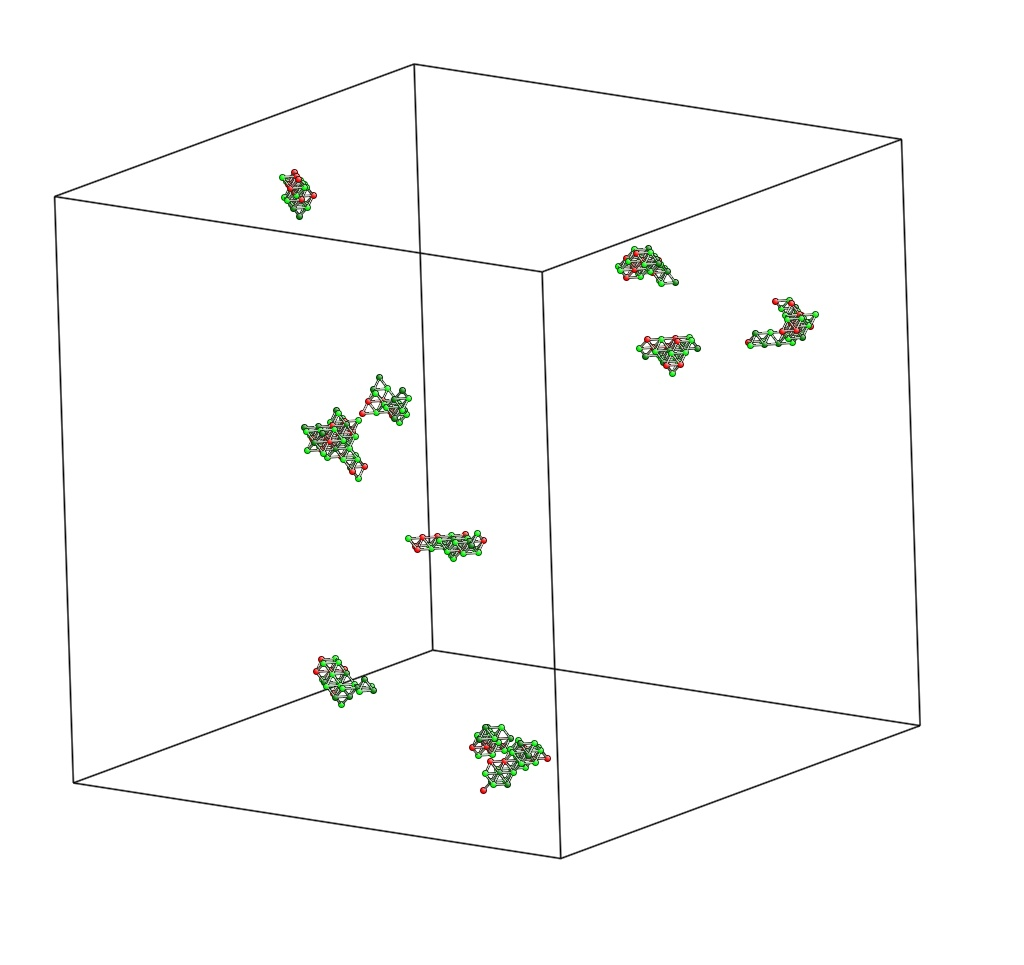
\includegraphics[width=0.49\linewidth]{Chap5/plots/cluster_illu_1.jpg}}
  \subfigure[]{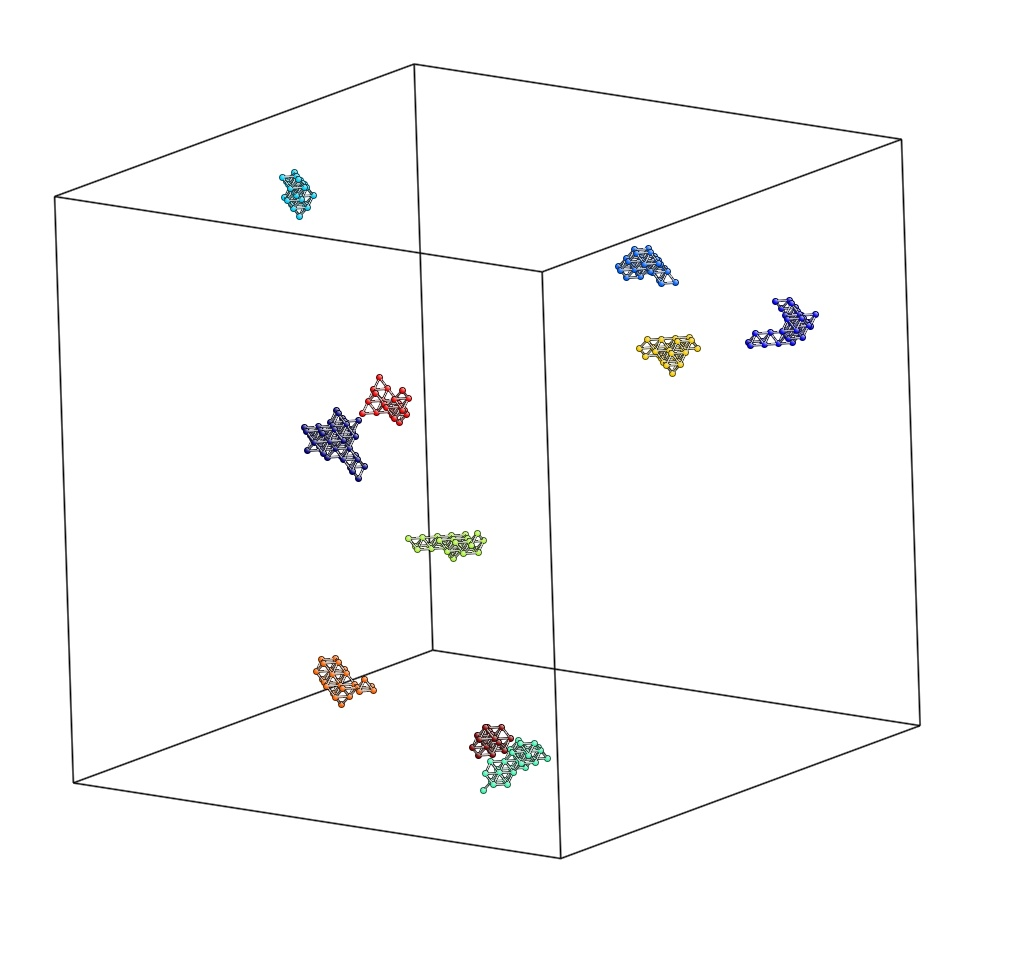
\includegraphics[width=0.49\linewidth]{Chap5/plots/cluster_illu_2.jpg}}
\caption[Atomistic pictures of the top 10 largest clusters by size via cluster searching algorithm.]{Atomistic pictures of the top 10 largest clusters by size via cluster searching algorithm from a snapshot during a \ac{kMC} simulation. (a) Atomistic pictures of clusters coloring in atom species. Light green, dark green, and red atoms are Al, Mg, and Zn, respectively. (b) Atomistic pictures of clusters coloring in cluster id. The color mapping from dark blue to red is ranked by the cluster size in descending order. Small gray sticks are bonds between atoms.}
\label{Chap:Al/Vac:fig:illu_cluster}
\end{figure}
\endgroup


In order to better analyzing our results, we have to use a visualization method to characterize clusters. A cluster is a set of connected atoms, each of which is within the range of one or more other atoms from the same cluster. Thus, any two atoms from the same cluster are connected by a continuous path consisting of steps fulfilling the selected neighboring criterion. Adversely, two atoms are not considered in the same cluster if there is no continuous path on the neighbor network leading from one particle to the other. We choose between the distance-based neighbor criterion, in which case two atoms are considered neighbors if they are within the neighbor list of each other. However, in our case, all the atoms are on the lattice, so the method described above does not work. It simply finds one huge cluster containing all the atoms. Therefore, we use the method described in Algorithm \ref{algo:cluster}. We show one typical result in Figure \ref{Chap:Al/Vac:fig:illu_cluster} from a snapshot during a \ac{kMC} simulation. To better visualize the details of clusters,  only the top ten clusters are shown. 


\begin{figure}[!htb]
  \centering
  \begin{minipage}{.75\linewidth}
    \begin{algorithm}[H]
      \caption{Cluster Searching Algorithm}\label{algo:cluster}
      \begin{algorithmic}[1]
        \State remove all the solvent atoms (Al for example).
        \State assign an initial cluster id, ($cid = -1$), to all the atoms.
        \State set $count = 0$.
        \For {i in all the solute atoms}
          \If {$cid_i = -1$}
            \State set $cid_i = count$.
            \State \ac{BFS} in the neighbor list of atom i to find other solute atoms if cluster size is greater than $size_{critical}$ and set their $cid = count$.
            \State add their first nearest neighbor solvent atoms (Al for example) back if the solvent atom have more than $bond_{critical}$ solute first nearest neighbors and set their $cid = count$.
            \State $count += 1$.
          \EndIf
        \EndFor
        \State then clusters can be sorted according to any customized methods, by cluster size, element ratios for examples.
      \end{algorithmic}
    \end{algorithm}
  \end{minipage}
\end{figure}


\subsection{Benchmark of Al-Mg-Zn Clusters}
\label{Chap:Al/Vac:benchmark}
For the \ac{kMC} simulations, (30$\times$30$\times$30) supercell containing 108,000 atoms were used. 3240 Mg atoms, 1700 Zn atoms, and 1 vacancy atom were randomly chosen among 108,000 atoms. This setup corresponds to $\sim$3 atom. \% of Mg, $\sim$2 atom. \% of Zn and a vacancy concentration of $\sim$ 1$\times10^{-5}$. We used \ac{LSKMC} algorithm to boost the simulation. After around $\sim$5.5 seconds of simulation, clusters size and the ratio of Mg/Zn converged to a local minimum of a very initial stage of the multiple-stage clustering process. As shown in Figure \ref{Chap:Al/Vac:fig:Al_Mg_Zn_benchmark} (a), the size of Al-Mg-Zn clusters are converging to a $\sim$2400 atoms size using Algorithm \ref{algo:cluster} with $size_{critical}$ of 3 and $bond_{critical}$ of 3. If tighter criteria($size_{critical}$ of 4 and $bond_{critical}$ of 4) were used, much fewer atoms can be identified as forming clusters and number of atoms in clusters converges to a much smaller value of $\sim$1000. Although the tighter criteria offset cluster sizes by almost 1000, both two setups follow the same trend and converge after several seconds.

\begingroup
\begin{figure}[!ht]
  \centering
  \subfigure[]{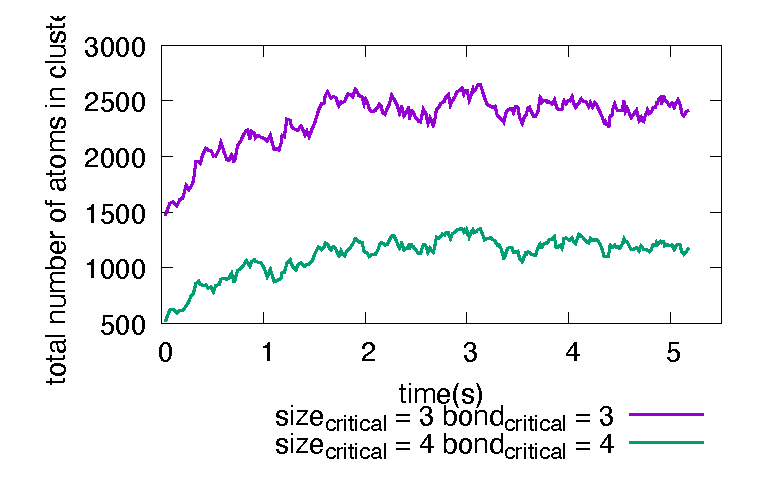
\includegraphics[width=0.8\linewidth]{Chap5/plots/size_control.eps}}
  \subfigure[]{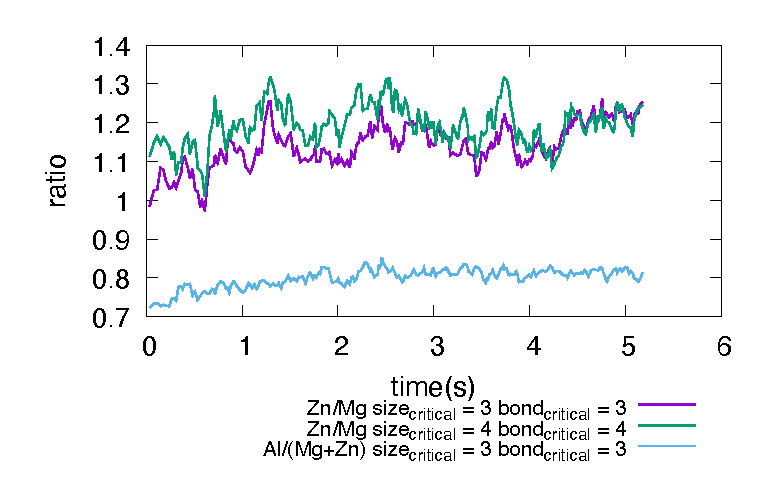
\includegraphics[width=0.8\linewidth]{Chap5/plots/ratio_control.eps}}
\caption[Size changes and ratio changes vs. time for $\sim$5.5 seconds. ]{Size changes and ratio changes vs. time for $\sim$5.5 seconds. Subplot. (a) the change of cluster size including Al, Mg, and Zn atoms. (b) the change of Al/(Mg+Zn) and Zn/Mg ratio. The purple line uses $size_{critical}$ of 3 and $bond_{critical}$ of 3. The green line uses $size_{critical}$ of 4 and $bond_{critical}$ of 4. The change of cluster size and Zn/Mg ratio follow a similar trend and converge after around $\sim$4 seconds.}
\label{Chap:Al/Vac:fig:Al_Mg_Zn_benchmark}
\end{figure}
\endgroup

And in Figure \ref{Chap:Al/Vac:fig:Al_Mg_Zn_benchmark} (b), we plotted the ratio of Zn/Mg within identified clusters. Also, two different criteria were tested. When the bonding criterion ($bond_{critical}$) was set to 4, very little Al atoms are counted as clusters, resulting in a very low Al/(Mg+Zn) ratio; therefore, we did not plot it here. Again, both setups trend similarly for Zn/Mg ratio and converge around 1.25. This ratio of Zn-rich clusters is comparable to the early stage solute clusters reported in \cite{liu2020formation}. Thus, in the following part of this chapter, $size_{critical}$ of 3 and $bond_{critical}$ of 3 were used for the cluster analyses. 

Atomistic pictures of those clusters can be found in Figure \ref{Chap:Al/Vac:fig:sens_control}. In addition, the distribution of cluster sizes is provided in Figure \ref{Chap:Al/Vac:fig:size_distr}. With cluster size frequencies, it becomes easier to identify how many clusters are stable. In Figure \ref{Chap:Al/Vac:fig:size_distr} (a) and (b) we compared the size distribution of a Al-Mg-Zn system evolving for 5 seconds and 22 seconds. Both configurations at 5 and 22 seconds follow a Poisson distribution pattern. In Figure \ref{Chap:Al/Vac:fig:long}, we also observed the number of Al, Mg, and Zn atoms in all identified clusters and the number of Mg-Zn bonds across the structure (both matrix and clusters) for the first 22 seconds. After the initial 1 or 2 seconds, these two descriptors became steady and oscillated around 2500 and 1200, respectively.


\newpage
\begingroup
\begin{figure}[!ht]
  \centering
  \subfigure[cluster]{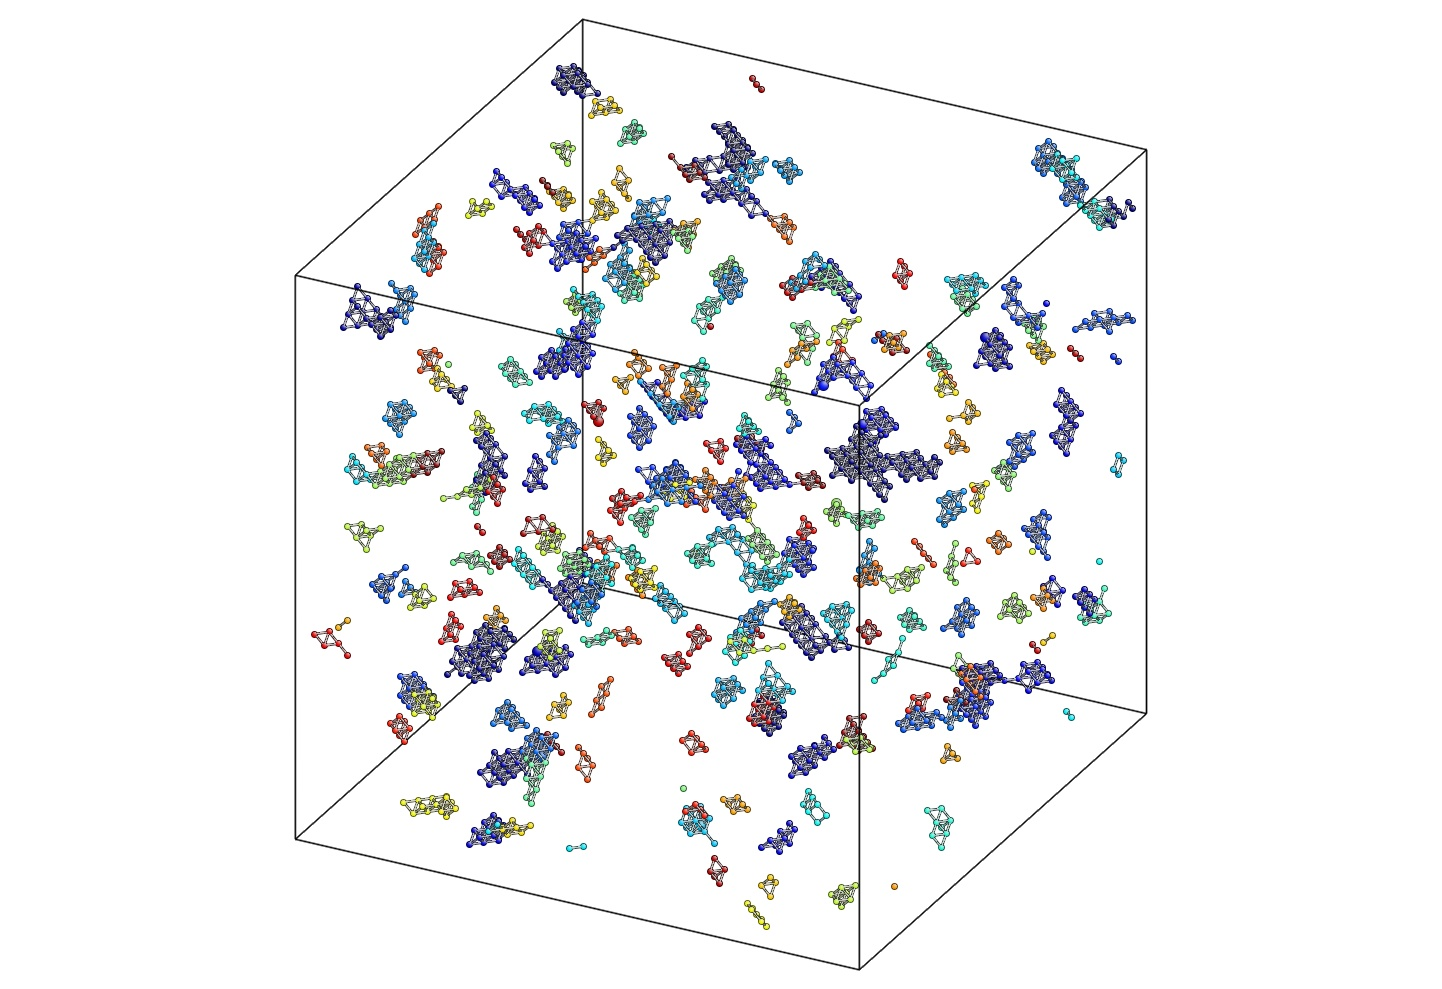
\includegraphics[width=0.75\linewidth]{Chap5/plots/cluster_id_jpg/00000.jpg}}
  \subfigure[species]{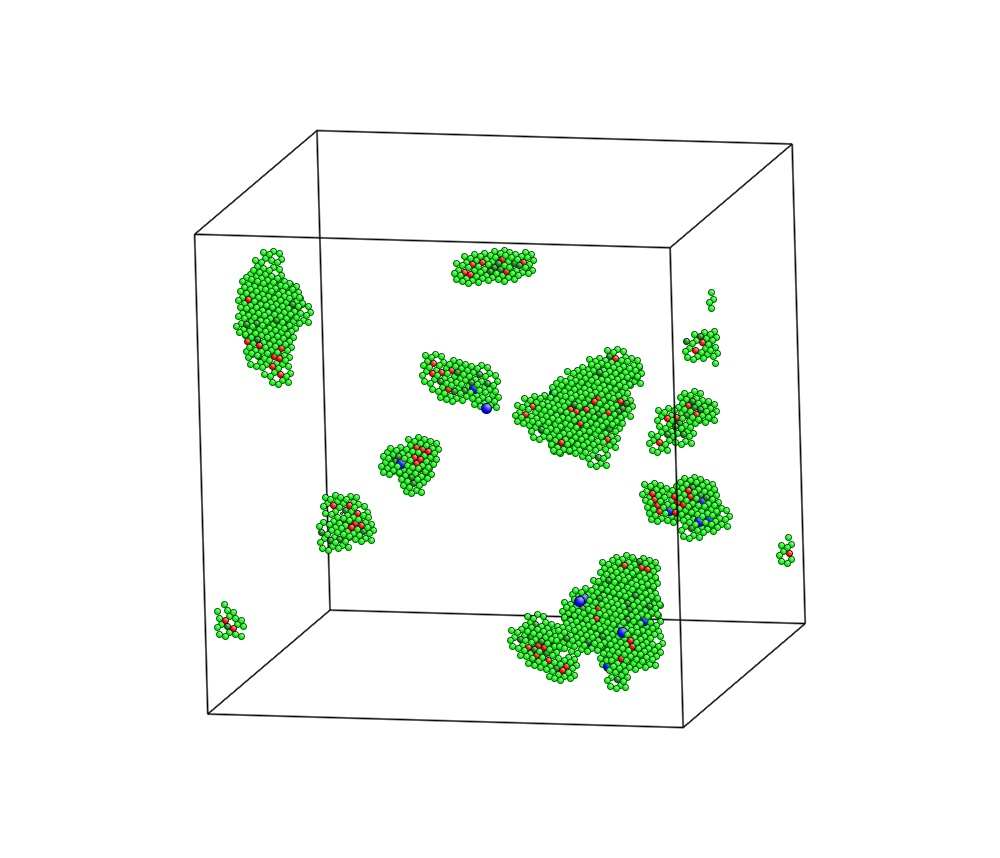
\includegraphics[width=0.75\linewidth]{Chap5/plots/element_jpg/00000.jpg}}
\caption[Atomistic pictures of 108,000 atoms for the control group of the sensitivity test.]{Atomistic pictures of 108,000 atoms for control group, corresponding to setup \#0 in Table \ref{Chap:Al/Vac:tab:pseudo1}. Subplot. (a) is colored by cluster size. The color mapping from dark blue to red is ranked by the cluster size in descending order. Subplot. (b) is colored by atom species. Light green, dark green, red, and blue atoms are Al, Mg, Zn, and pseudo atoms respectively. Small gray sticks are bonds between atoms.}
\label{Chap:Al/Vac:fig:sens_control}
\end{figure}
\endgroup

\begingroup
\begin{figure}[!ht]
  \centering
  \subfigure[]{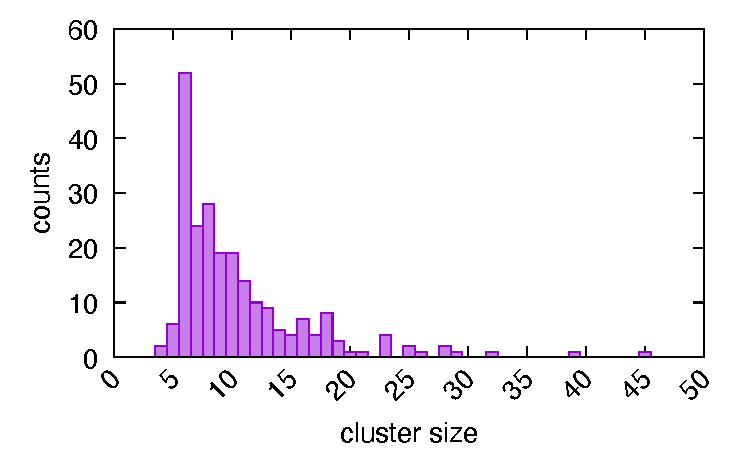
\includegraphics[width=0.65\linewidth]{Chap5/plots/size_dist_5.pdf}}
  \subfigure[]{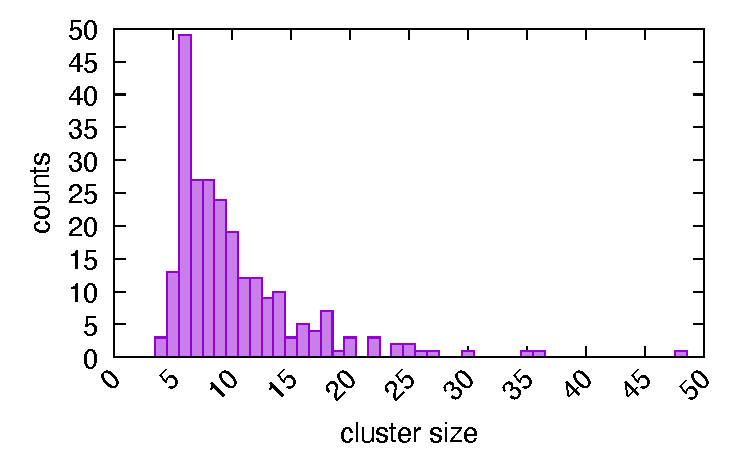
\includegraphics[width=0.65\linewidth]{Chap5/plots/size_dist_22.pdf}}
\caption[Size distribution of identified clusters at 5 seconds and 22 seconds.]{Size distribution of identified clusters at 5 seconds in plot (a) and 22 seconds in plot (b).}
\label{Chap:Al/Vac:fig:size_distr}
\end{figure}
\endgroup


\begingroup
\begin{figure}[!ht]
  \centering
  \subfigure[]{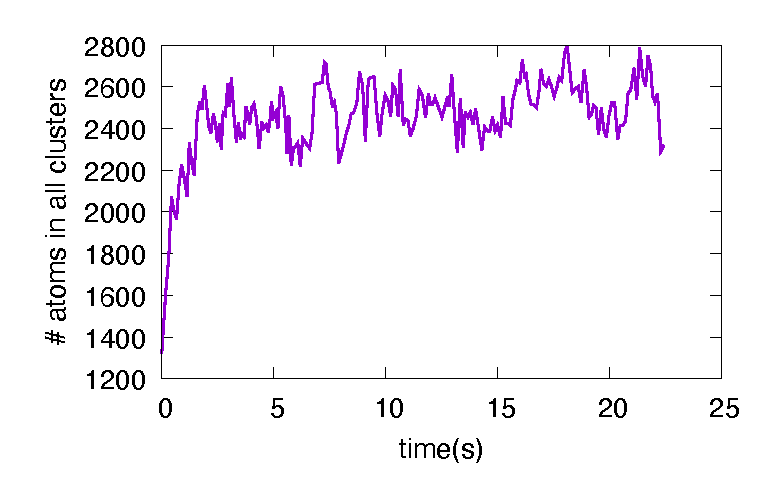
\includegraphics[width=0.65\linewidth]{Chap5/plots/size_control_long.eps}}
  \subfigure[]{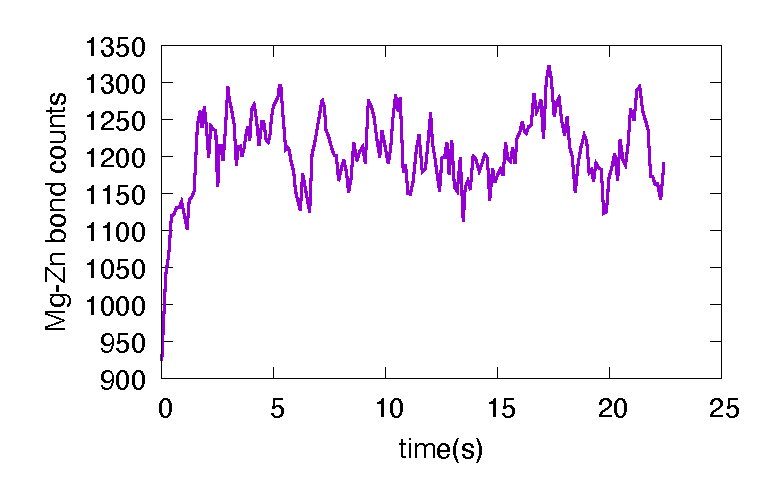
\includegraphics[width=0.65\linewidth]{Chap5/plots/bond_MgZn_long.eps}}
\caption[Cluster size and Mg-Zn bonds change for the first 22 seconds.]{Cluster size and Mg-Zn bonds change for the first 22 seconds. (a) The number of Al, Mg, and Zn atoms in all identified clusters vs. time. (b) The number of Mg-Zn bonds across the structure (both matrix and clusters) vs. time.}
\label{Chap:Al/Vac:fig:long}
\end{figure}
\endgroup





\subsection{Searching for Potential Elements that Can Slow Down Precipitate Hardening}
\label{Chap:Al/Vac:pseudo}
Similar to the idea of searching ``anchor'' elements in Chapter \ref{Chap:Ag/ZnO:section:anchor}, we will first use \ac{kMC} simulation with some pseudo-atoms (denoted as ``X'') to study their effects on the early stage clustering. In this study, we have Al atoms as solvent atoms, and Mg, Zn, and X atoms as solute atoms. For these simulations, (30$\times$30$\times$30) supercell containing 108,000 atoms were used. 3240 Mg atoms, 1700 Zn atoms, 1080 X atoms, and 1 vacancy atom were randomly chosen among 108,000 atoms. This setup corresponds to $\sim$3 atom. \% of Mg, $\sim$2 atom. \% of Zn, $\sim$1 atom. \% of X, and a vacancy concentration of $\sim$1$\times10^{-5}$. Note that this concentration is set to conduct the sensitivity tests only. This $\sim$1 atom. \% is not a trace amount value, but it can help to boost the effects of pseudo-atoms. To tune the properties of pseudo atoms, we can change the effects of different elements on vacancy migration barriers to the pseudo-atoms, as well as barriers to other elements. We leverage this by adding an offset to the vacancy migration barrier calculated from \ac{NN} model via Equation \ref{Chap:Al/Vac:eq:offset} . The amount of the offset is determined by counting first neighbor bonding of X-Al, X-Mg, and X-Zn, via Equation \ref{Chap:Al/Vac:eq:offset_calculation}:
\begin{subequations}
\begin{align}
{E_a}^{actual} & = {E_a}^{NN} + \textit{offset} \label{Chap:Al/Vac:eq:offset} \\
\textit{offset} & = \varepsilon_{i-X} * ( n_{i-X}^{final} - n_{i-X}^{init}) \label{Chap:Al/Vac:eq:offset_calculation}
\end{align}
\end{subequations}
where ${E_a}^{NN}$ is the energy obtained by the neural network prediction of treating element ``X'' as the solvent element Al. $i$ is the atomic type of the swapped atom that the vacancy would jump to, which can be Al, Mg, or Zn. $\varepsilon_{i-X}$ quantify the pseduo-atom effects on the vacancy migration barrier $offset$ in Equation \ref{Chap:Al/Vac:eq:offset_calculation} by simple bonding counting method. $n_{i-X}^{init}$ and $n_{i-X}^{final}$ are the number of $i-X$ bonds between the swapped atom $i$ and the pseudo-atom $X$ in its first nearest neighbor before and after the vacancy migration, respectively. For example, if $\varepsilon_{Al-X} = 0.01$ that means a new Al-X pair in the final state after the vacancy migration increases the vacancy migration barrier by a positive 0.01 eV.

The right-hand side of Equation \ref{Chap:Al/Vac:eq:offset} can be divided into two parts. The first part, which is \ac{NN} potential part, can be seen as a more comprehensive bond counting model \cite{soisson1996monte} base on the pair interactions of Al-Al, Al-Mg, Al-Zn, and Mg-Zn, plus cross interactions or higher-ordered angular contributions. The second part of the right-hand side can be seen as first-order bond counting of Al-X, Mg-X, and Zn-X. As a qualitative study, first order pair-wise interaction of the unknown pseudo-atoms should be sufficient. Then the target is to find an element ``X'' that can change the vacancy migration barrier of Vac-i by roughly the amount of $\varepsilon_{i-X}$ to achieve the optimal effects to slow down the solute clustering during the natural aging in Al-Mg-Zn alloys. In the future, with the optimized $\varepsilon_{i-X}$ values for slowing down solute clustering, we can use \ac{DFT} with \ac{NEB} to search for potential realistic chemical elements that can change the vacancy migration barriers according to Equations \ref{Chap:Al/Vac:eq:offset} and \ref{Chap:Al/Vac:eq:offset_calculation} with the optimized $\varepsilon_{i-X}$.

To setup the simulation for sensitivity tests, we use \ac{LSKMC} method with $step_{critical}$ of 25,000 steps and $E_{critical}$ of 0.3 eV. After around 5 to 6 seconds simulations, we can already tell the differences of cluster size obviously. As discussed above, we tuned parameters of $\varepsilon_{i-X}$ for $i \in {Al, Mg, Zn}$ in Equation \ref{Chap:Al/Vac:eq:offset_calculation}. Detailed setup is listed in Table \ref{Chap:Al/Vac:tab:pseudo1}. All the sensitivity tests can be divided into four groups: the control group with all $\varepsilon_{i-X}$ = 0 (Setup \#0 in Table \ref{Chap:Al/Vac:tab:pseudo1}), the Al group with only $\varepsilon_{Al-X}$ $\ne$ 0 (Setup \#1 and \#2 in Table \ref{Chap:Al/Vac:tab:pseudo1}), the Mg group with only $\varepsilon_{Mg-X}$ $\ne$ 0 (Setup \#3 and \#4 in Table \ref{Chap:Al/Vac:tab:pseudo1}), and the Zn group with only $\varepsilon_{Zn-X}$ $\ne$ 0 (Setup \#5 and \#6 in Table \ref{Chap:Al/Vac:tab:pseudo1}). Their corresponding final snapshots of clusters for the control group, Al group, Mg group, and Zn group can be found in Figure \ref{Chap:Al/Vac:fig:sens_control}, \ref{Chap:Al/Vac:fig:sens_Al}, \ref{Chap:Al/Vac:fig:sens_Mg}, and \ref{Chap:Al/Vac:fig:sens_Zn}, respectively. 


\begin{table}[!htbp]
\centering
\caption[Sensitivity analyses of different $\varepsilon_{i-X}$.]{Sensitivity analyses of different $\varepsilon_{i-X}$ in Equation \ref{Chap:Al/Vac:eq:offset_calculation}. In the table, the number of different element types in all identified clusters are listed using $size_{critical}$ of 3(4) and $bond_{critical}$ of 3(4).}
\label{Chap:Al/Vac:tab:pseudo1}
\begin{tabular}{cccccccc}
\\
\hline
\hline
setup & $\varepsilon_{Al-X}$  & $\varepsilon_{Mg-X}$  & $\varepsilon_{Zn-X}$ & Al counts & Mg counts & Zn counts & pseudo counts\\
\hline
0 &  0.00    &  0.00       &  0.00 & 1078(230) & 588(421)  &  737(524)  & 11(4)                \\
1 &  0.05    &  0.00       &  0.00 & 1229(270) &  689(434) &   778(549) & 0(0)                \\
2 & -0.05    &  0.00       &  0.00 & 1407(312) & 922(753)  & 1017(871)  & 406(252)                \\
3 &  0.00    &  0.05       &  0.00 & 1442(353) & 1121(919) & 794(620)   & 292(171)                \\
4 &  0.00    & -0.05       &  0.00 & 1012(215) &  588(407) &  638(463)  & 5(1)                \\
5 &  0.00    &  0.00       &  0.05 & 1407(395) & 522(407)  & 1325(1164) & 385(253)                \\
6 &  0.00    &  0.00       & -0.05 & 1042(222) &  590(363) &  730(489)  & 3(0)                \\

\hline
\hline
\end{tabular}
\end{table}

\begingroup
\begin{figure}[!ht]
  \centering
  \subfigure[$\varepsilon_{Al-X} = 0.05$, cluster]{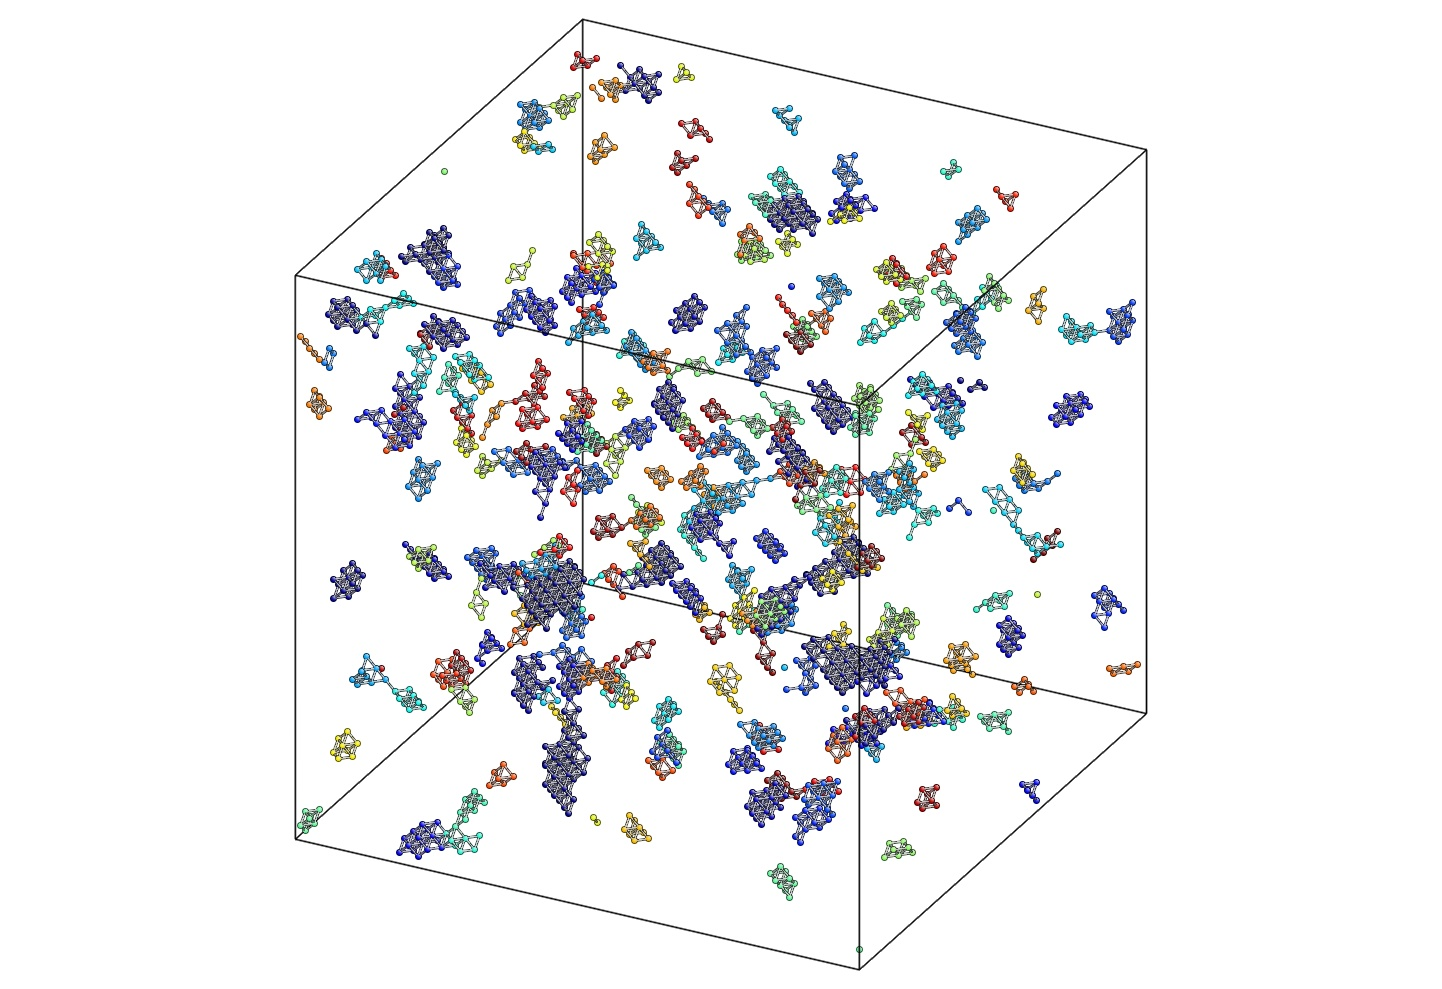
\includegraphics[width=0.49\linewidth]{Chap5/plots/cluster_id_jpg/00001.jpg}}
%   \subfigure[control, cluster]{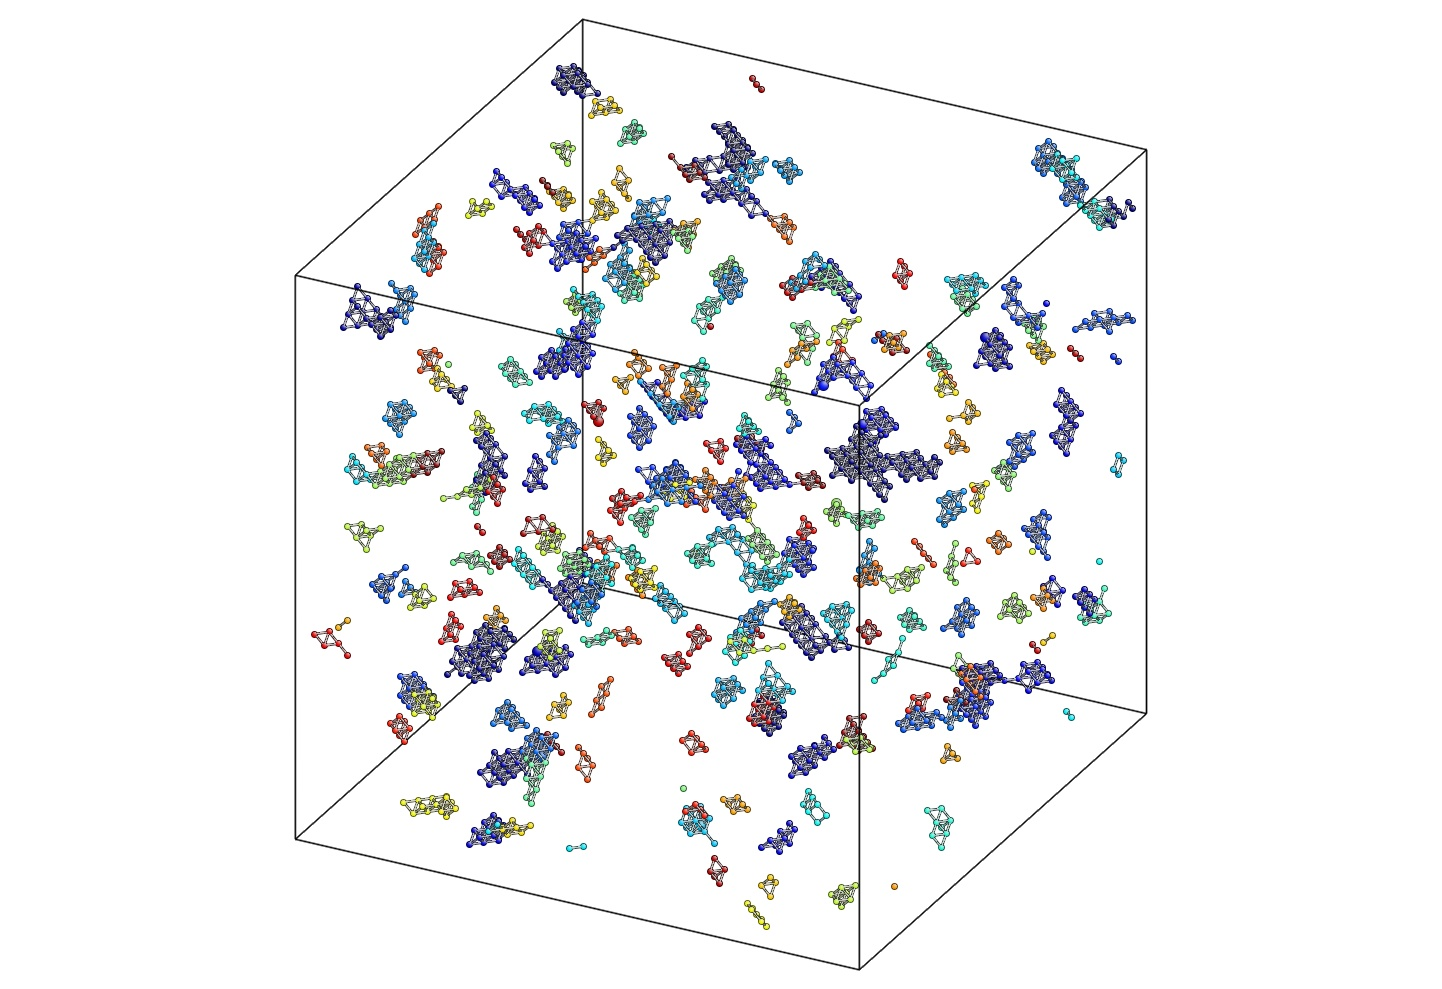
\includegraphics[width=0.49\linewidth]{Chap5/plots/cluster_id_jpg/00000.jpg}}
  \subfigure[$\varepsilon_{Al-X} = -0.05$, cluster]{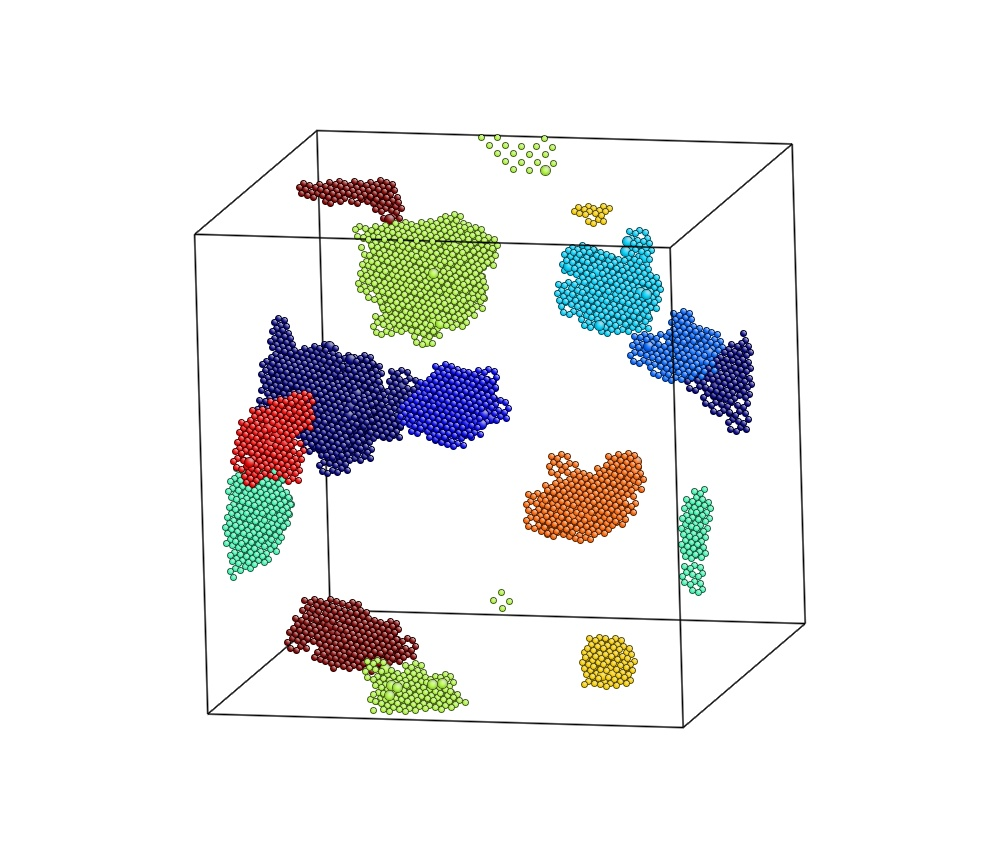
\includegraphics[width=0.49\linewidth]{Chap5/plots/cluster_id_jpg/00002.jpg}}
  \subfigure[$\varepsilon_{Al-X} = 0.05$, species]{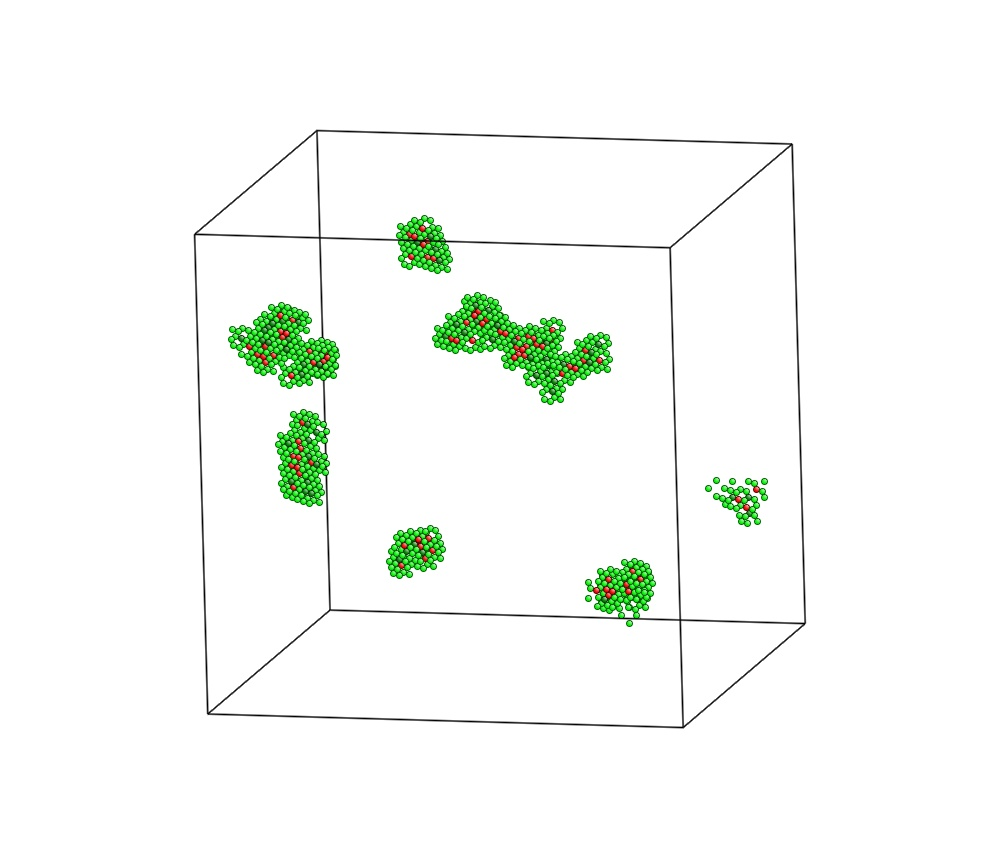
\includegraphics[width=0.49\linewidth]{Chap5/plots/element_jpg/00001.jpg}}
%   \subfigure[control, species]{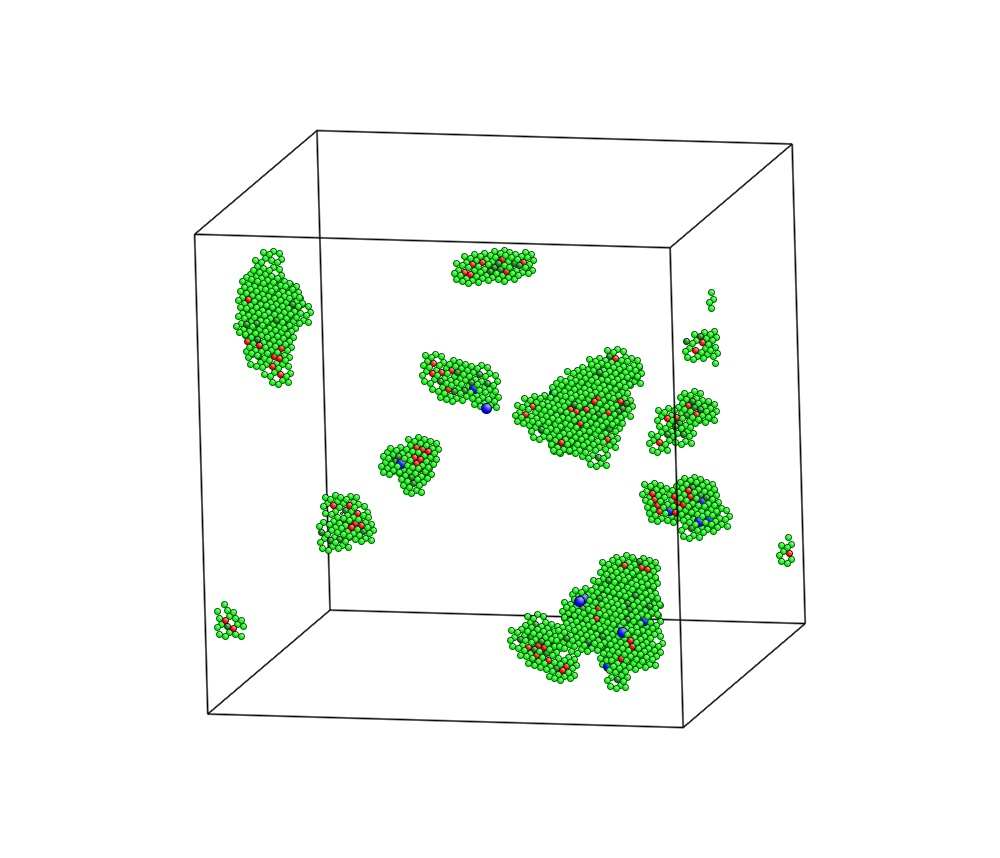
\includegraphics[width=0.49\linewidth]{Chap5/plots/element_jpg/00000.jpg}}
  \subfigure[$\varepsilon_{Al-X} = -0.05$, species]{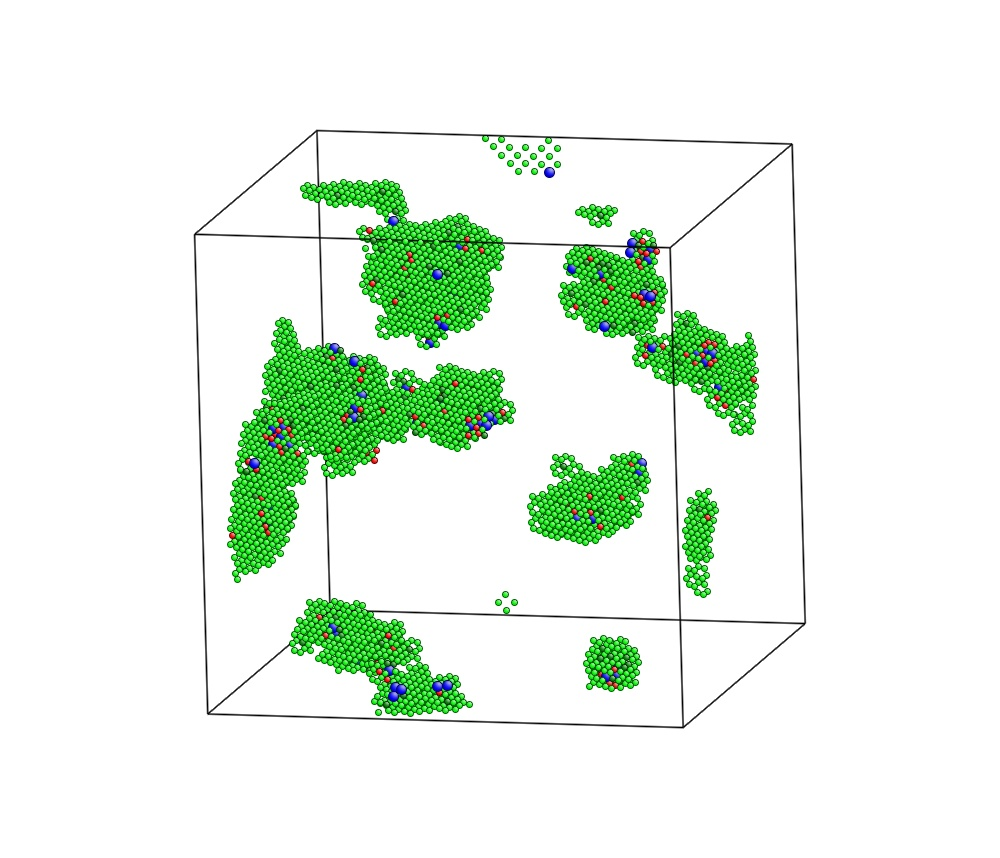
\includegraphics[width=0.49\linewidth]{Chap5/plots/element_jpg/00002.jpg}}

\caption[Atomistic pictures of 108,000 atoms for $\varepsilon_{Al-X}$ sensitivity test.]{Atomistic pictures of 108,000 atoms for $\varepsilon_{Al-X}$ sensitivity test using $size_{critical}$ of 3 and $bond_{critical}$ of 3. (a), (c) : $\varepsilon_{Al-X} = 0.05$, which is setup \#1 in Table \ref{Chap:Al/Vac:tab:pseudo1}. (b), (d) : $\varepsilon_{Al-X} = -0.05$, which is setup \#2 in Table \ref{Chap:Al/Vac:tab:pseudo1}. (a) and (c) are colored by cluster size. The color mapping from dark blue to red is ranked by the cluster size in descending order. (b) and (d) are colored by atom species. Light green, dark green, red, and blue atoms are Al, Mg, Zn, and pseudo atoms respectively. And small gray sticks are bonds between atoms.}
\label{Chap:Al/Vac:fig:sens_Al}
\end{figure}
\endgroup


\begingroup
\begin{figure}[!ht]
  \centering
  \subfigure[$\varepsilon_{Mg-X} = 0.05$, cluster]{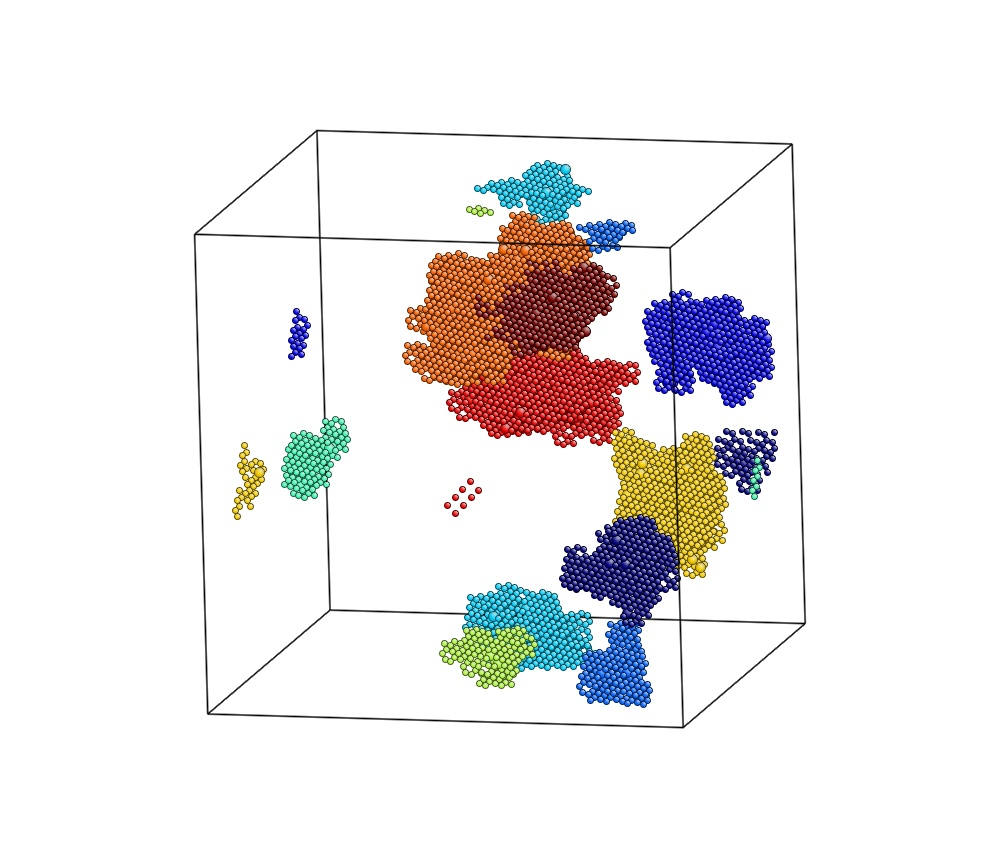
\includegraphics[width=0.49\linewidth]{Chap5/plots/cluster_id_jpg/00003.jpg}}
%   \subfigure[control]{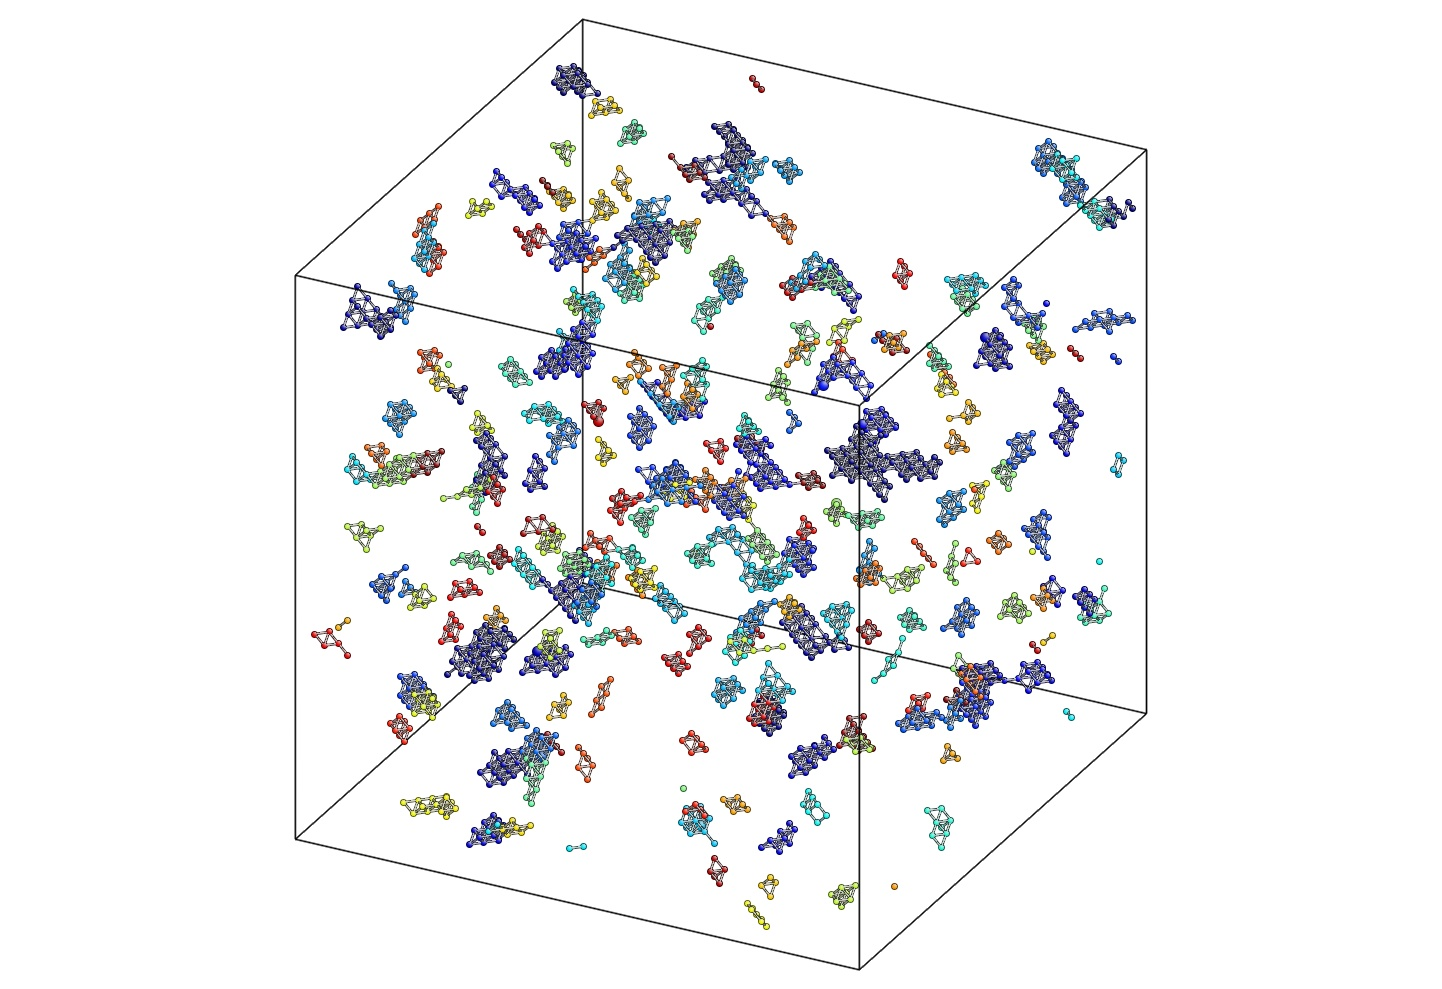
\includegraphics[width=0.32\linewidth]{Chap5/plots/cluster_id_jpg/00000.jpg}}
  \subfigure[$\varepsilon_{Mg-X} = -0.05$, cluster]{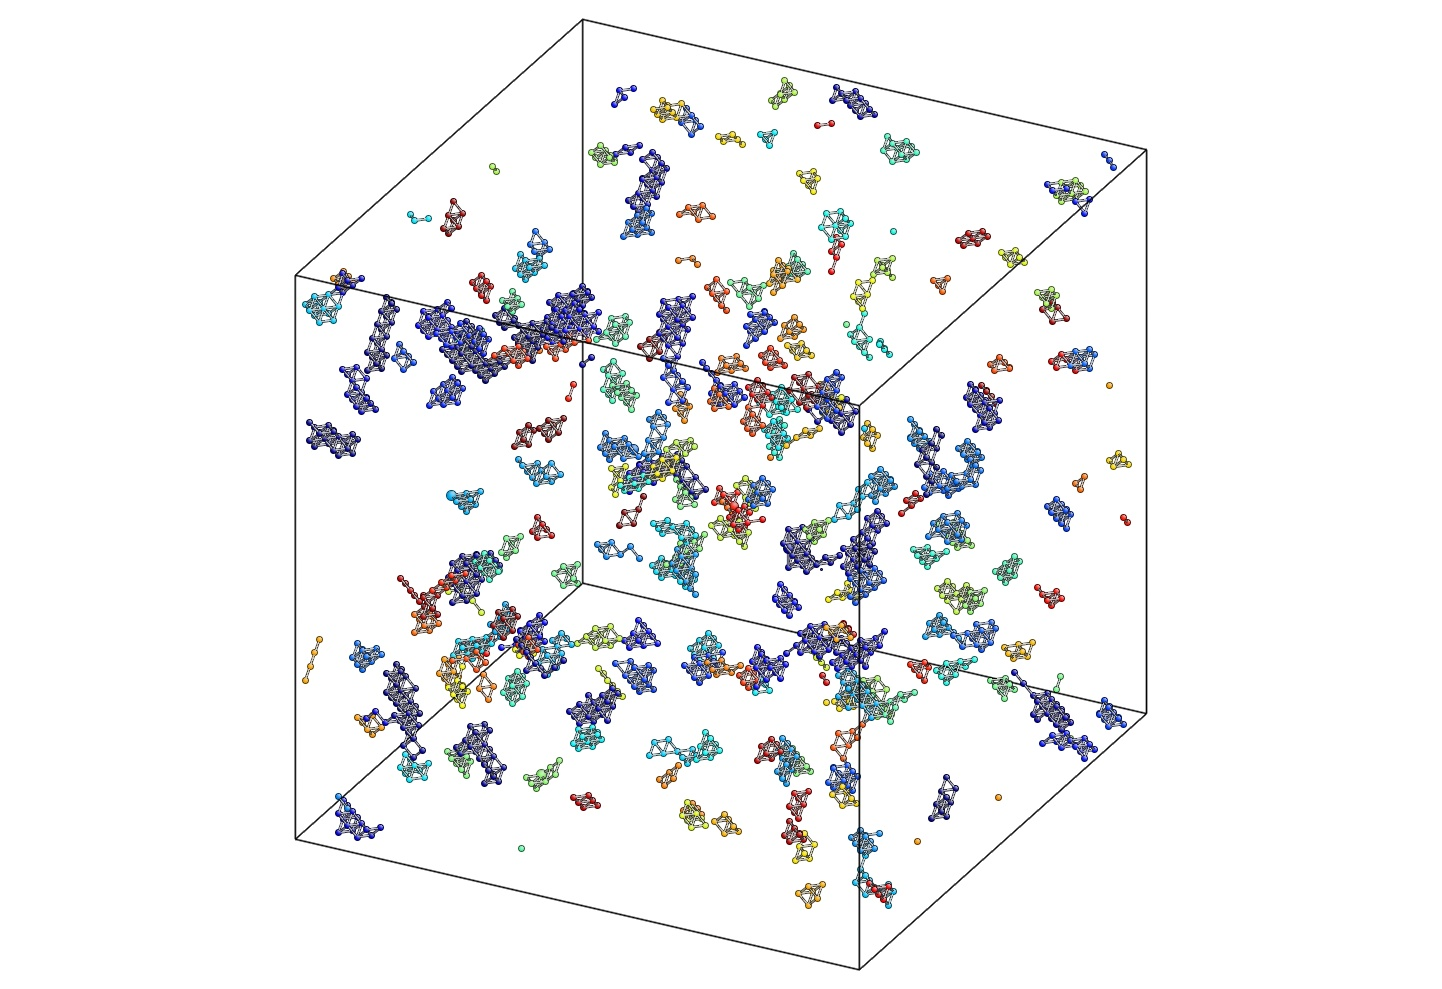
\includegraphics[width=0.49\linewidth]{Chap5/plots/cluster_id_jpg/00004.jpg}} \\
  \subfigure[$\varepsilon_{Mg-X} = 0.05$, species]{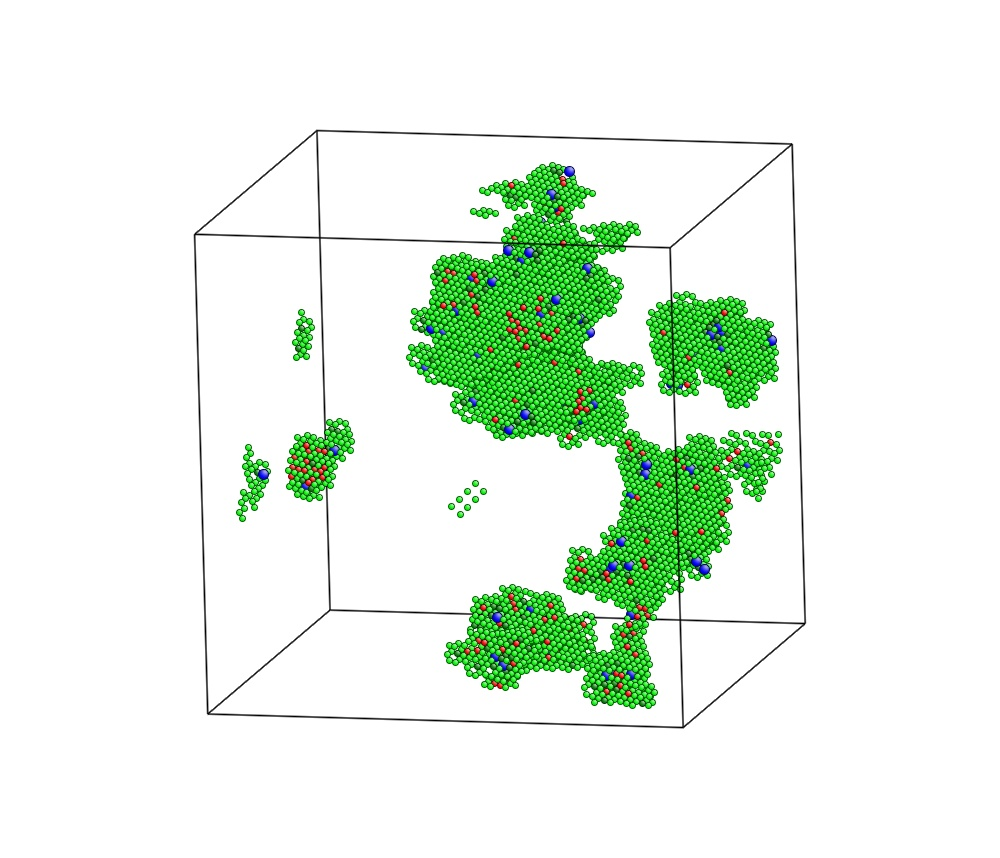
\includegraphics[width=0.49\linewidth]{Chap5/plots/element_jpg/00003.jpg}}
%   \subfigure[control]{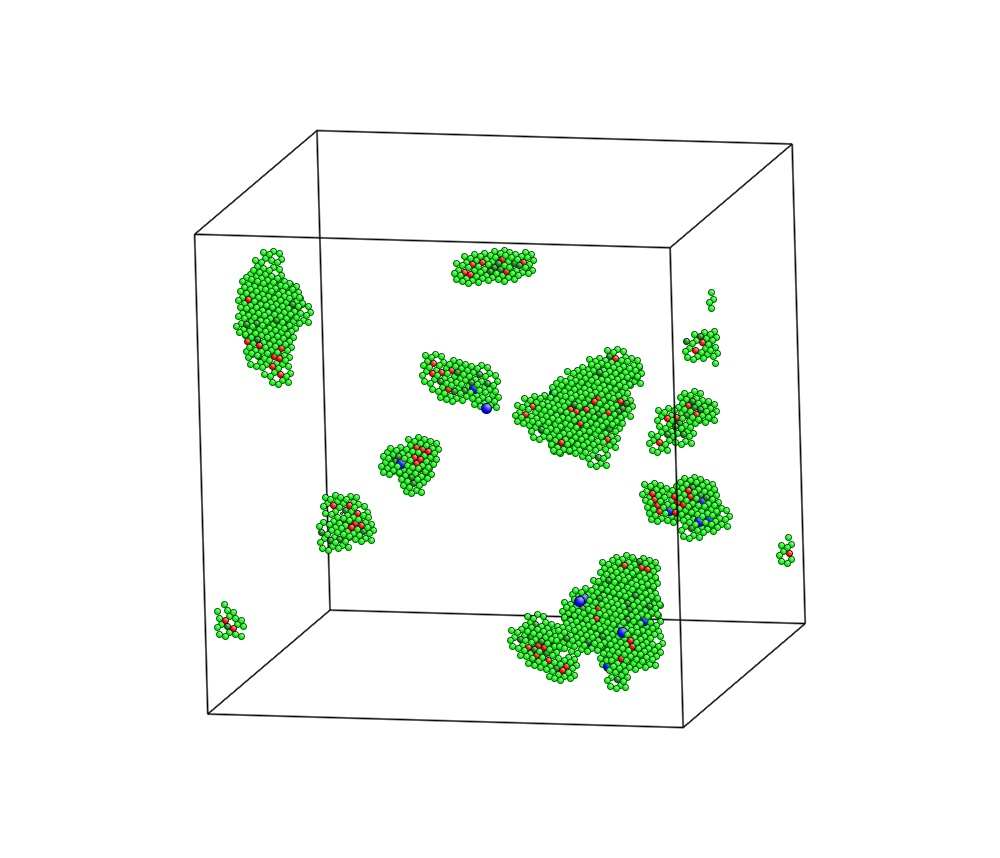
\includegraphics[width=0.32\linewidth]{Chap5/plots/element_jpg/00000.jpg}}
  \subfigure[$\varepsilon_{Mg-X} = -0.05$, species]{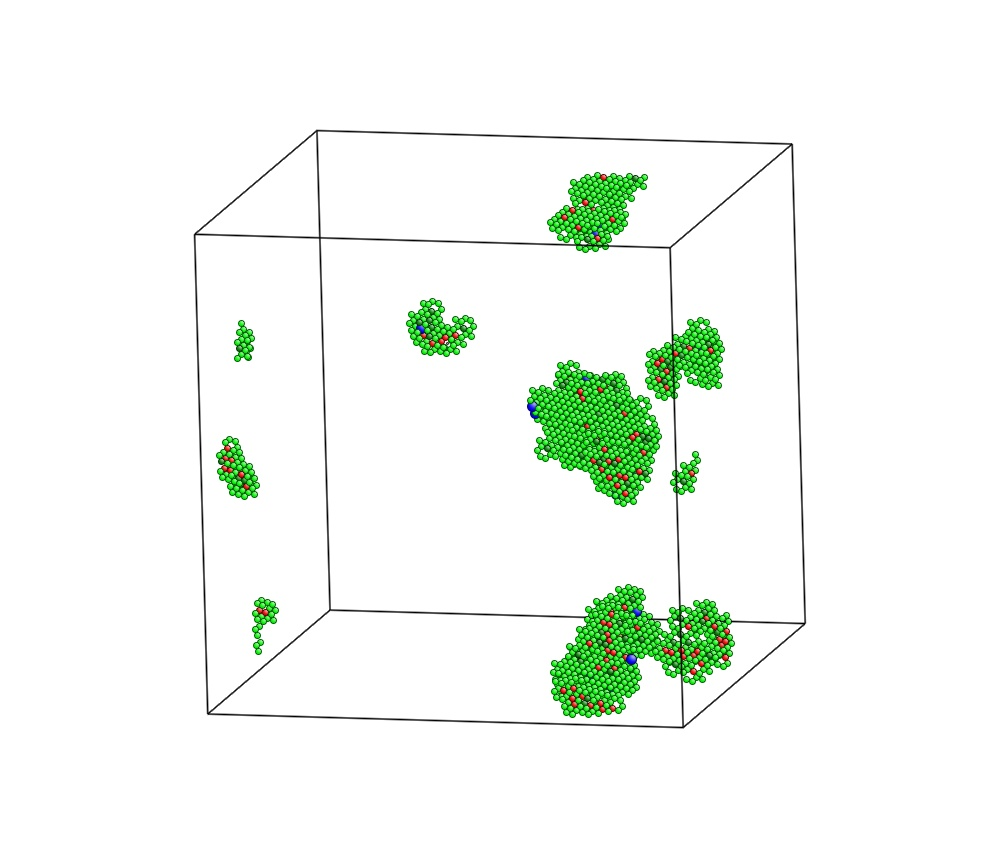
\includegraphics[width=0.49\linewidth]{Chap5/plots/element_jpg/00004.jpg}}

\caption[Atomistic pictures of 108,000 atoms for $\varepsilon_{Mg-X}$ sensitivity test.]{Atomistic pictures of 108,000 atoms for $\varepsilon_{Mg-X}$ sensitivity test using $size_{critical}$ of 3 and $bond_{critical}$ of 3. (a), (c) : $\varepsilon_{Mg-X} = 0.05$, which is setup \#3 in Table \ref{Chap:Al/Vac:tab:pseudo1}. (b), (d) : $\varepsilon_{Mg-X} = -0.05$, which is setup \#4 in Table \ref{Chap:Al/Vac:tab:pseudo1}. (a) and (c) are colored by cluster size. The color mapping from dark blue to red is ranked by the cluster size in descending order. (b) and (d) are colored by atom species. Light green, dark green, red, and blue atoms are Al, Mg, Zn, and pseudo atoms respectively. And small gray sticks are bonds between atoms.}
\label{Chap:Al/Vac:fig:sens_Mg}
\end{figure}
\endgroup


\begingroup
\begin{figure}[!ht]
  \centering
  \subfigure[$\varepsilon_{Zn-X} = 0.05$, cluster]{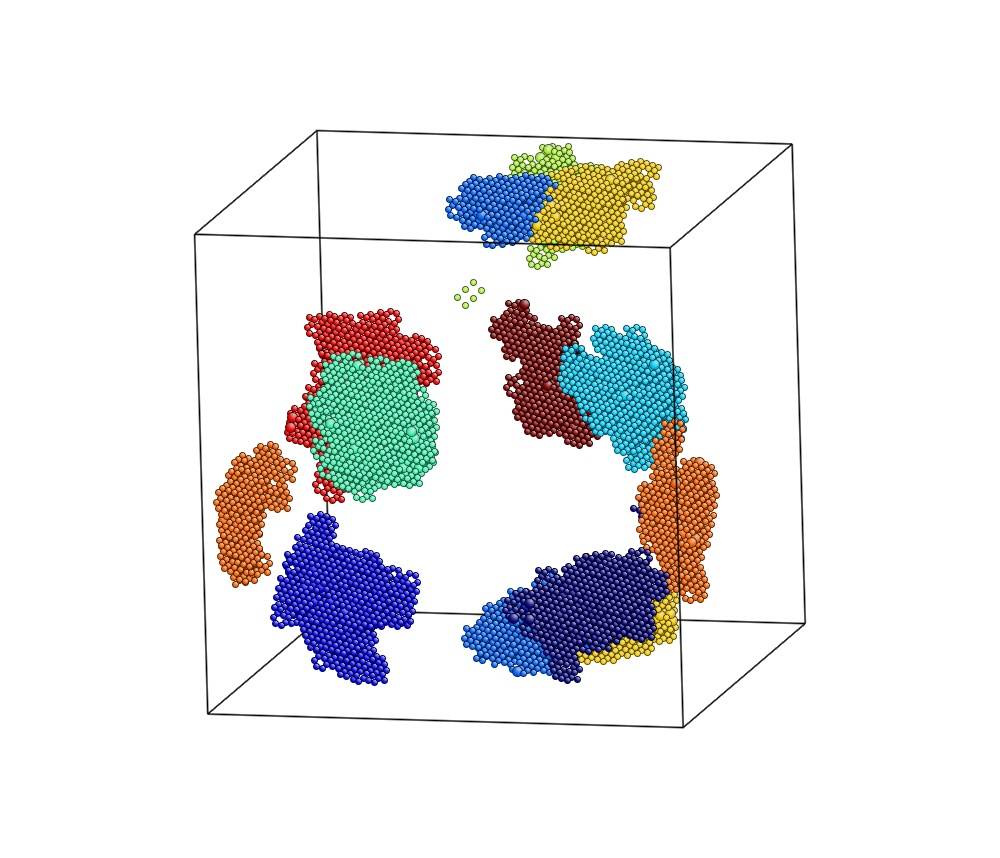
\includegraphics[width=0.49\linewidth]{Chap5/plots/cluster_id_jpg/00005.jpg}}
%   \subfigure[control]{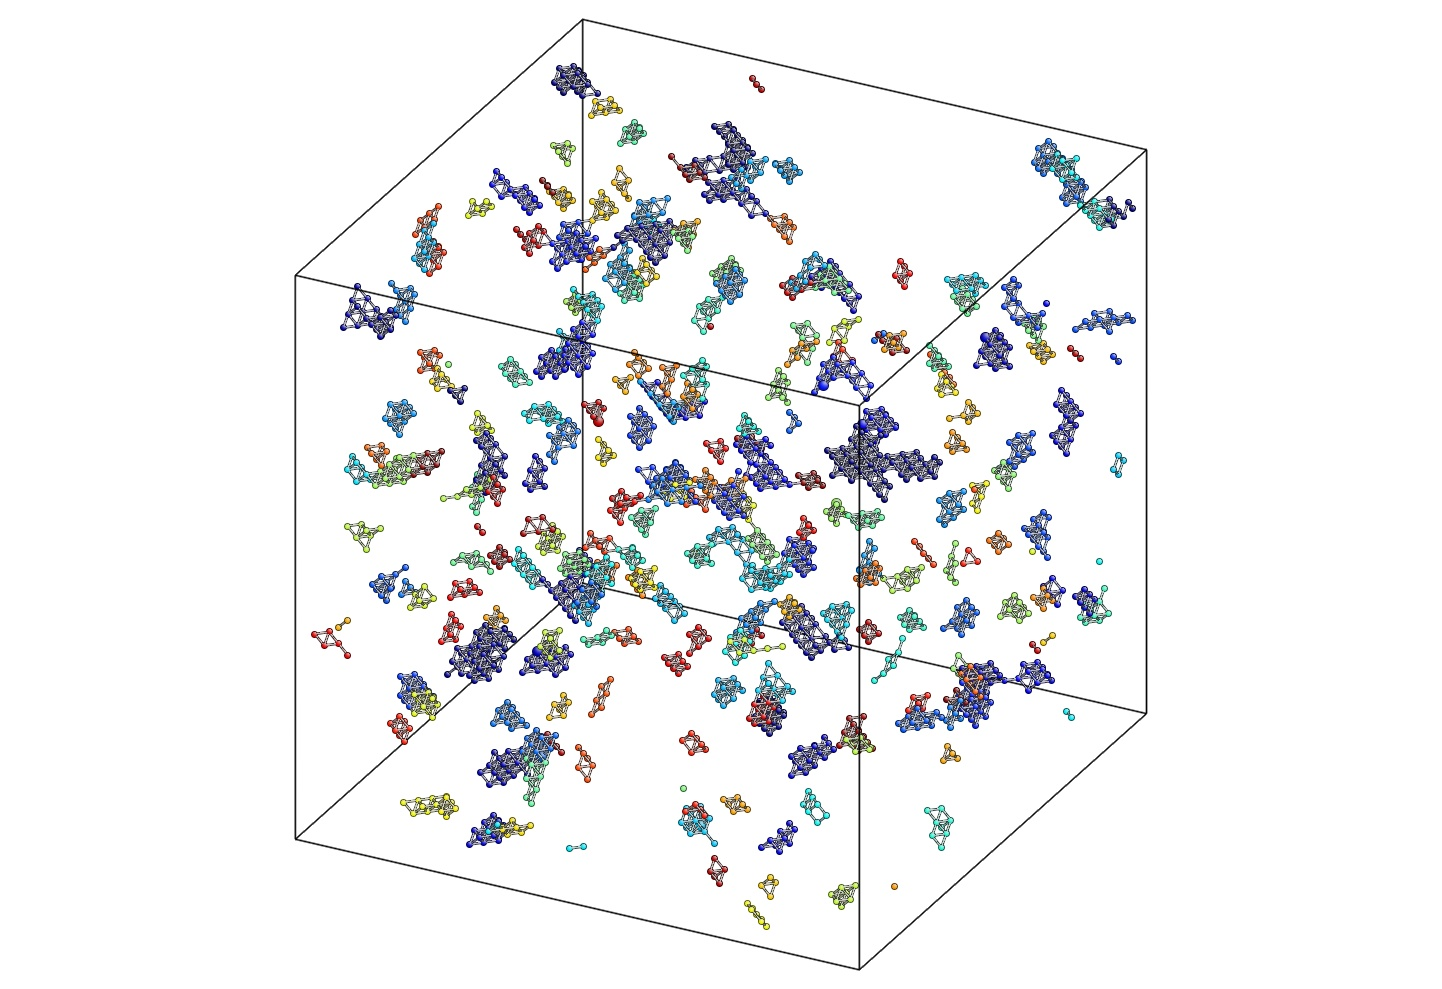
\includegraphics[width=0.32\linewidth]{Chap5/plots/cluster_id_jpg/00000.jpg}}
  \subfigure[$\varepsilon_{Zn-X} = -0.05$, cluster]{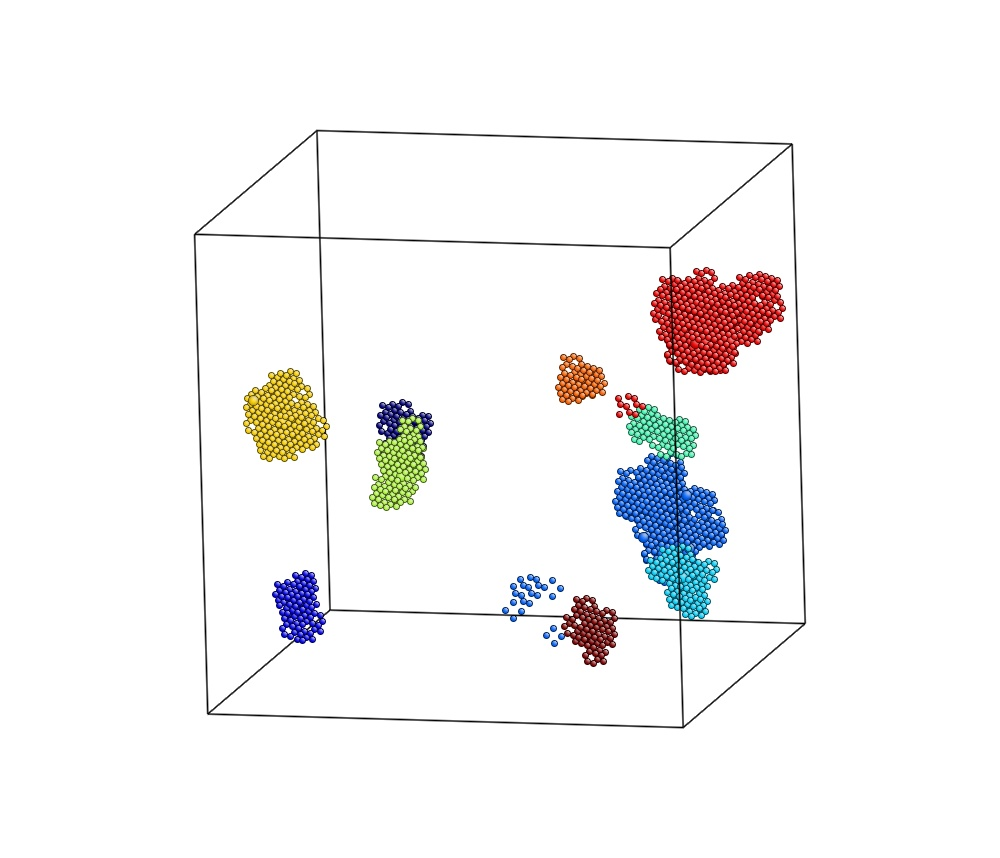
\includegraphics[width=0.49\linewidth]{Chap5/plots/cluster_id_jpg/00006.jpg}} \\
  \subfigure[$\varepsilon_{Zn-X} = 0.05$, species]{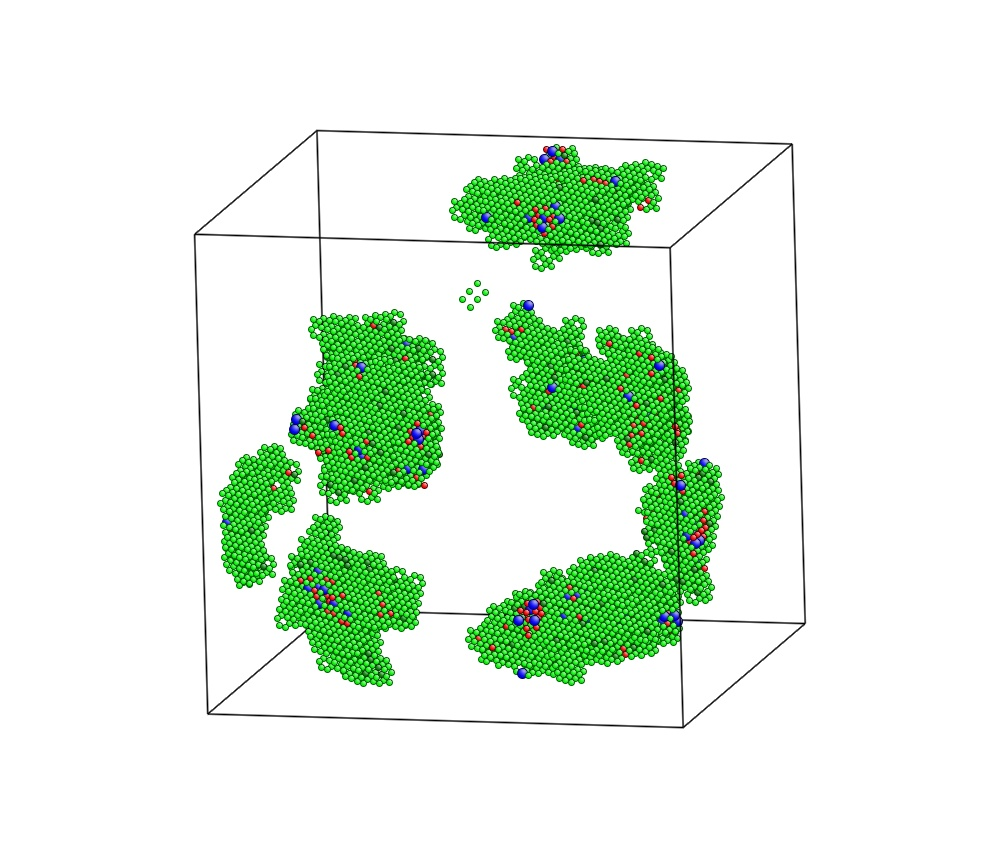
\includegraphics[width=0.49\linewidth]{Chap5/plots/element_jpg/00005.jpg}}
%   \subfigure[control]{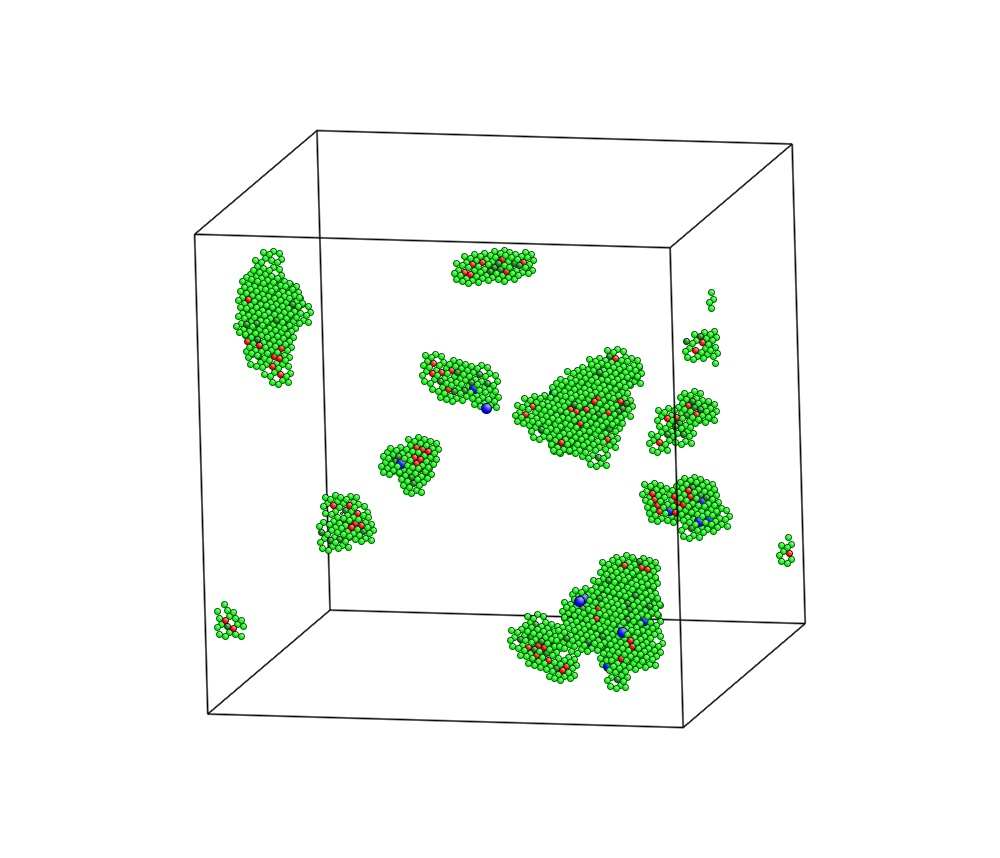
\includegraphics[width=0.32\linewidth]{Chap5/plots/element_jpg/00000.jpg}}
  \subfigure[$\varepsilon_{Zn-X} = -0.05$, species]{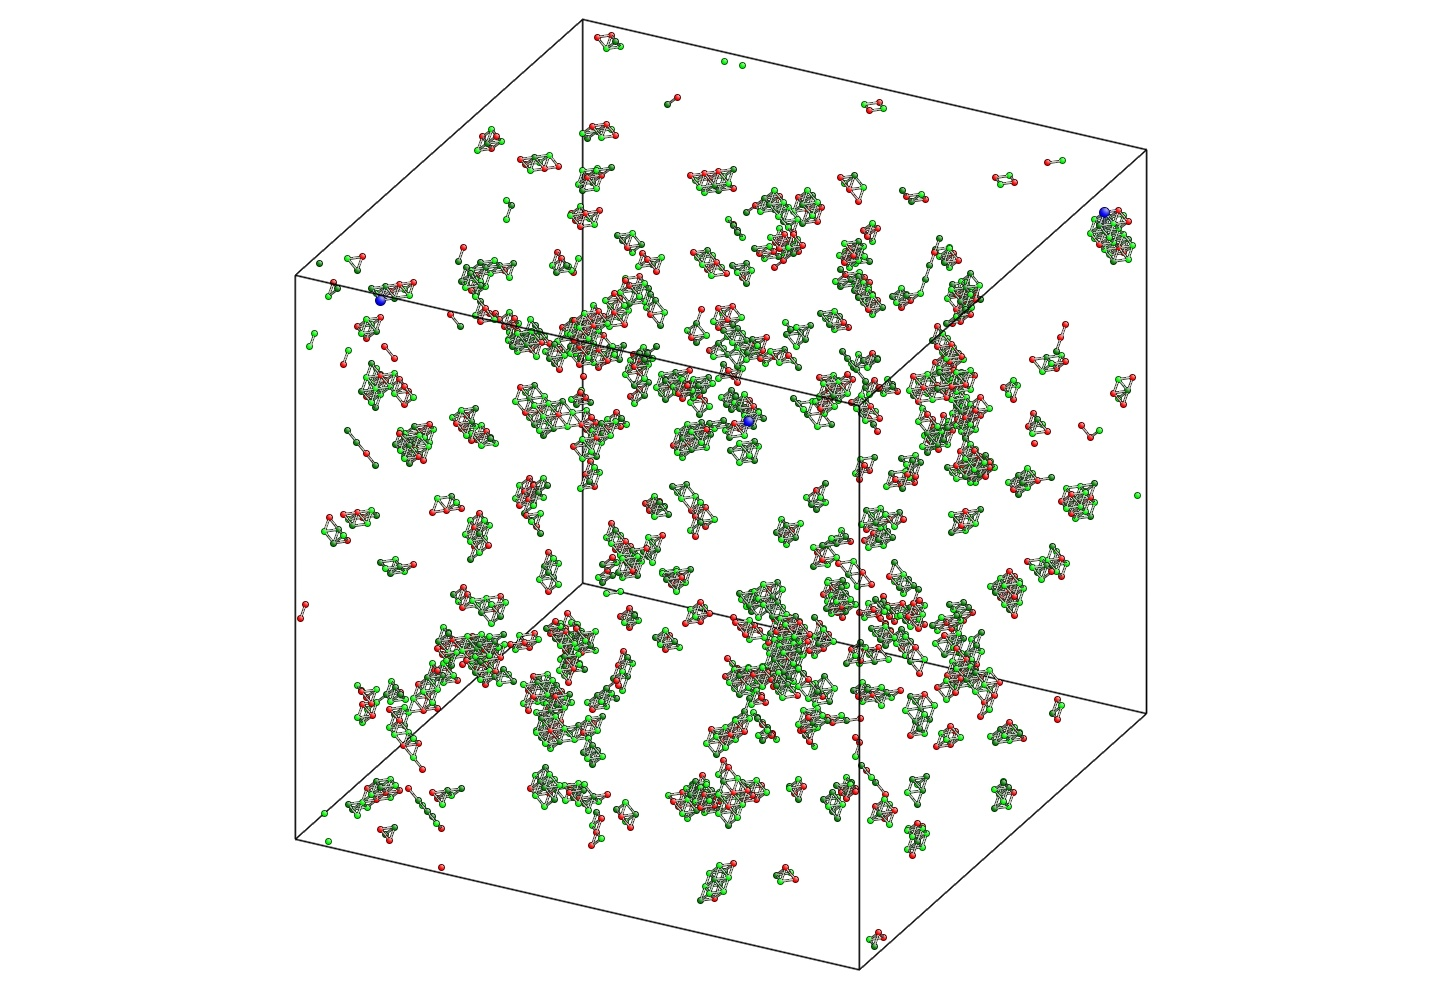
\includegraphics[width=0.49\linewidth]{Chap5/plots/element_jpg/00006.jpg}}

\caption[Atomistic pictures of 108,000 atoms for $\varepsilon_{Zn-X}$ sensitivity test.]{Atomistic pictures of 108,000 atoms for $\varepsilon_{Zn-X}$ sensitivity test using $size_{critical}$ of 3 and $bond_{critical}$ of 3. (a), (c) : $\varepsilon_{Zn-X} = 0.05$, which is setup \#5 in Table \ref{Chap:Al/Vac:tab:pseudo1}. (b), (d) : $\varepsilon_{Zn-X} = -0.05$, which is setup \#6 in Table \ref{Chap:Al/Vac:tab:pseudo1}. (a) and (c) are colored by cluster size. The color mapping from dark blue to red is ranked by the cluster size in descending order. (b) and (d) are colored by atom species. Light green, dark green, red, and blue atoms are Al, Mg, Zn, and pseudo atoms respectively. And small gray sticks are bonds between atoms.}
\label{Chap:Al/Vac:fig:sens_Zn}
\end{figure}
\endgroup



\newpage
\begingroup
\begin{figure}[!ht]
  \centering
  \subfigure[cluster size of Al Mg Zn X]{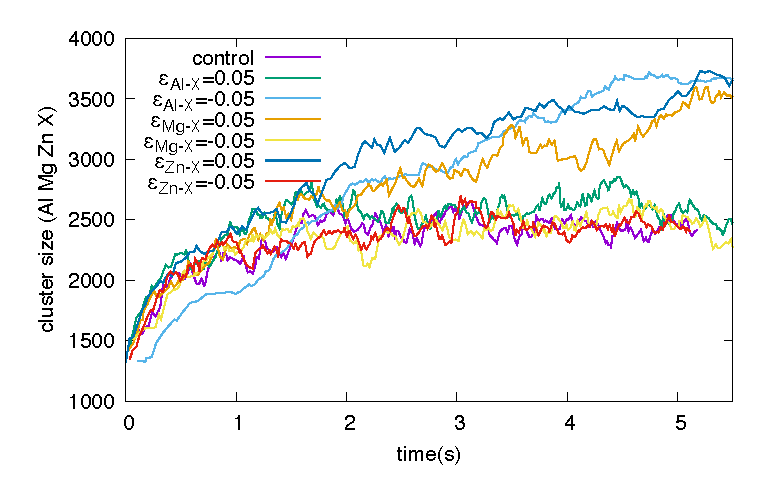
\includegraphics[width=0.6\linewidth]{Chap5/plots/size.eps}}
  \subfigure[cluster size of Al Mg Zn]{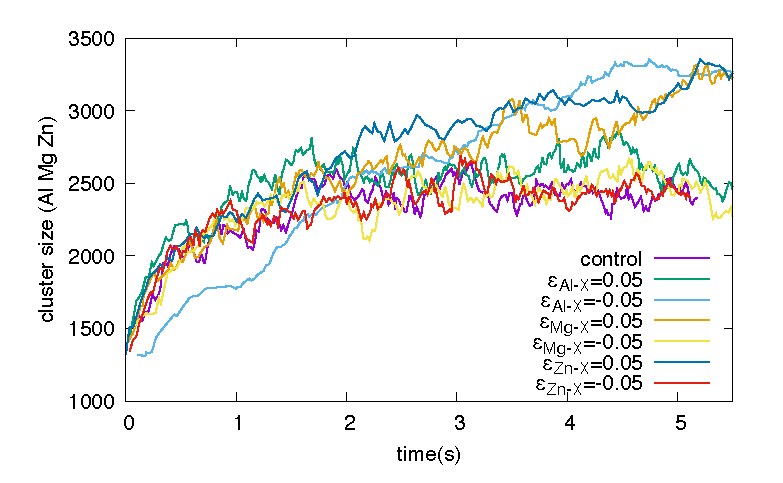
\includegraphics[width=0.6\linewidth]{Chap5/plots/size_noX.eps}}
\caption[Size changes of different clusters vs. time using $size_{critical}$ of 3 and $bond_{critical}$ of 3.]{Size changes of different clusters vs. time using $size_{critical}$ of 3 and $bond_{critical}$ of 3. Subplot. (a) is for all the atoms including pseudo atoms. (b) is for Al, Mg, and Zn only.}
\label{Chap:Al/Vac:fig:sens_cluster_size}
\end{figure}
\endgroup

In order to better visualize the change of structures and stoichiometry, we plotted the changes of the cluster sizes and the ratios between species in Figure \ref{Chap:Al/Vac:fig:sens_cluster_size} and \ref{Chap:Al/Vac:fig:sens_cluster_ratio}. In Figure \ref{Chap:Al/Vac:fig:sens_cluster_size}, cluster size change for the control group, Al group, Mg group, and Zn group are plotted. With and without considering pseudo-atoms in the clusters does not change the trend significantly. The purple line in Figure \ref{Chap:Al/Vac:fig:sens_cluster_size} represents the cluster size changes of the control group. Configurations with pseudo-atom having  $\varepsilon_{Al-X} = -0.05$, $\varepsilon_{Zn-X} = 0.05$, and $\varepsilon_{Mg-X} = 0.05$ have the ability to make clusters to grow much larger after around 2 second.  From Table \ref{Chap:Al/Vac:tab:pseudo1}, the number of Al, Mg, and Zn species in the identified clusters grow with the similar ratio relative to each other compared with those in the control group. However, their counterparts ($\varepsilon_{Al-X} = 0.05$, $\varepsilon_{Zn-X} = -0.05$, and $\varepsilon_{Mg-X} = -0.05$) cannot reduce the cluster size. Their curves behave similar to the control group.


\begingroup
\begin{figure}[!ht]
  \centering
  \subfigure[]{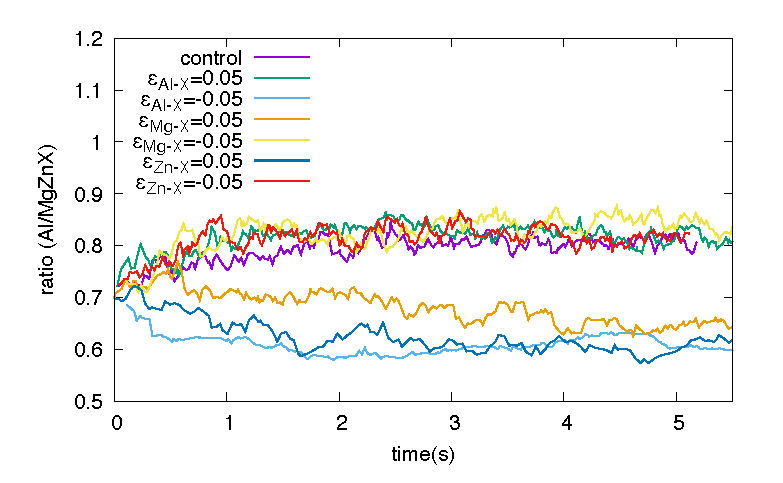
\includegraphics[width=0.49\linewidth]{Chap5/plots/ratio_Al-MgZnX.eps}}
  \subfigure[]{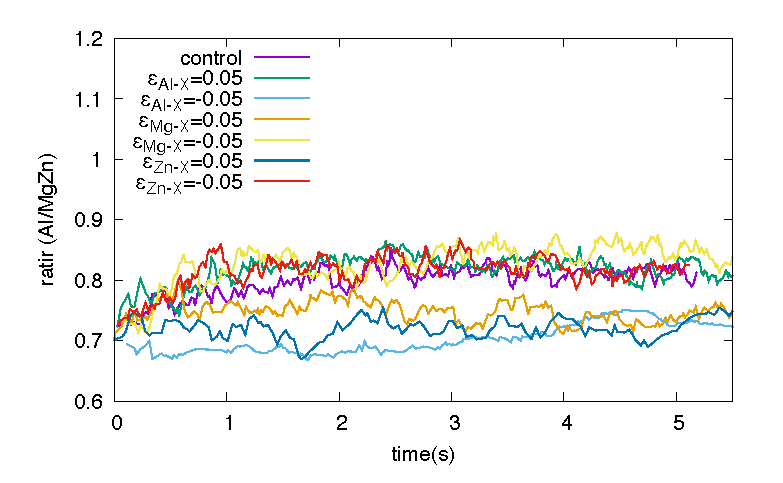
\includegraphics[width=0.49\linewidth]{Chap5/plots/ratio_Al-MgZn.eps}}
  \subfigure[]{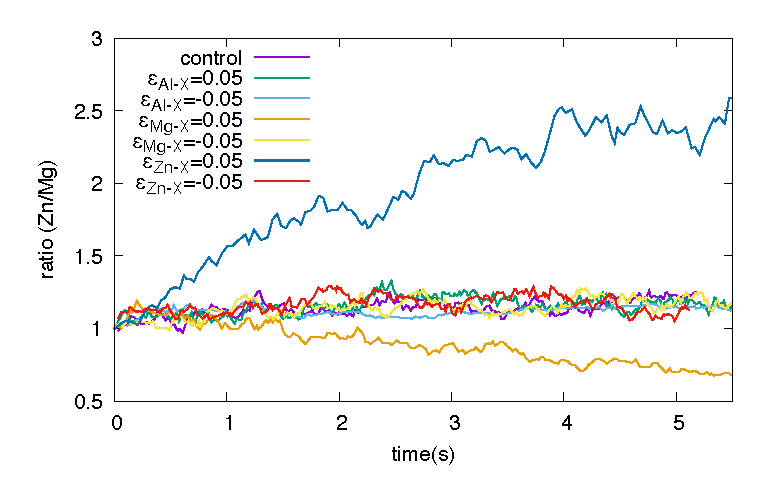
\includegraphics[width=0.49\linewidth]{Chap5/plots/ratio_Zn-Mg.eps}}
\caption[Ratio changes of different clusters vs. time using $size_{critical}$ of 3 and $bond_{critical}$ of 3.]{Ratio changes of different clusters vs. time using $size_{critical}$ of 3 and $bond_{critical}$ of 3. Subplot. (a) is for the ratio of all the Al atoms to the sum of Mg, Zn, and X atoms in the clusters. (b) is for the ratio of all the Al atoms to the sum of Mg and Zn atoms in the clusters. (c) is for Zn and Mg ratio in the clusters. X represents the pseudo-atom.}
\label{Chap:Al/Vac:fig:sens_cluster_ratio}
\end{figure}
\endgroup


\begingroup
\begin{figure}[!ht]
  \centering
  \subfigure[]{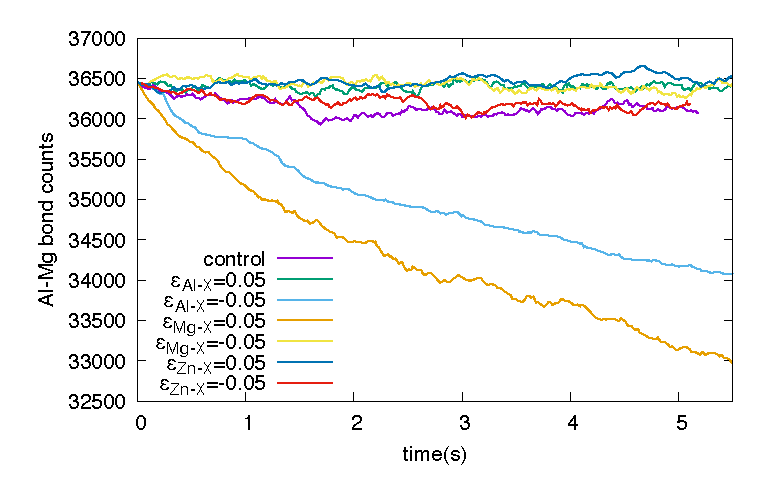
\includegraphics[width=0.49\linewidth]{Chap5/plots/bond_AlMg.eps}}
  \subfigure[]{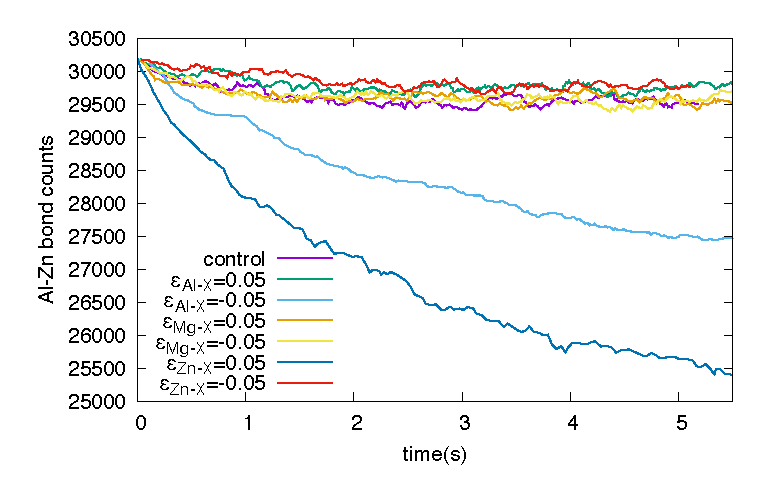
\includegraphics[width=0.49\linewidth]{Chap5/plots/bond_AlZn.eps}}
  \subfigure[]{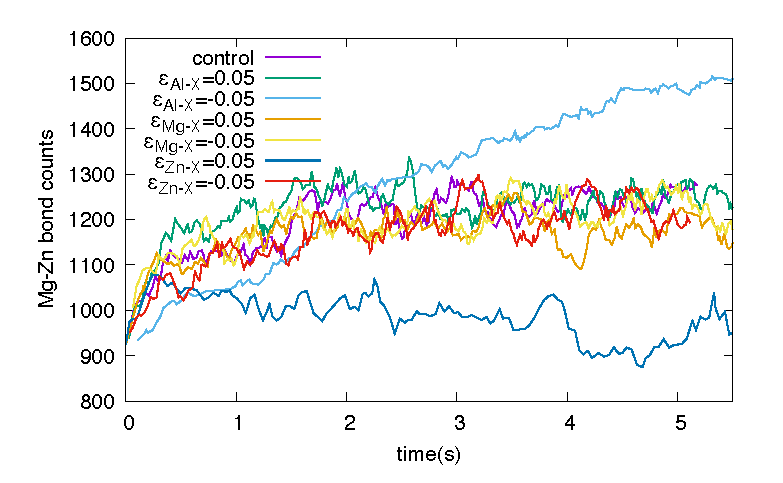
\includegraphics[width=0.49\linewidth]{Chap5/plots/bond_MgZn.eps}}
  \subfigure[]{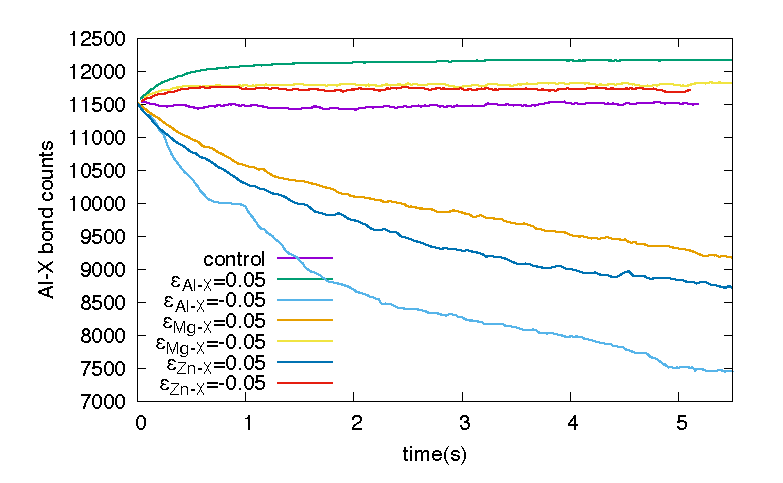
\includegraphics[width=0.49\linewidth]{Chap5/plots/bond_AlX.eps}}
  \subfigure[]{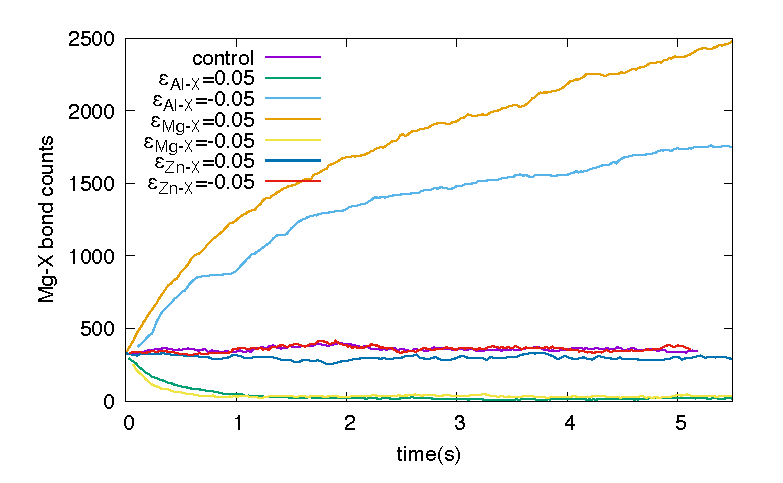
\includegraphics[width=0.49\linewidth]{Chap5/plots/bond_MgX.eps}}
  \subfigure[]{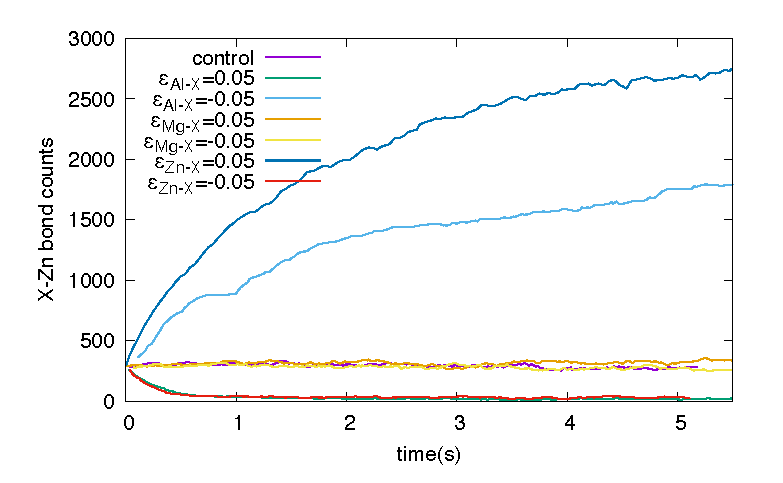
\includegraphics[width=0.49\linewidth]{Chap5/plots/bond_XZn.eps}}
\caption[Bonds between different species vs. time using $size_{critical}$ of 3 and $bond_{critical}$ of 3.]{Bonds between different species vs. time using $size_{critical}$ of 3 and $bond_{critical}$ of 3. (a), (b), (c), (d), (e), and (f) are for numbers of Al-Mg, Al-Zn, Mg-Zn, Al-X, Mg-X, and X-Zn bonds, respectively. X represents pseudo-atom.}
\label{Chap:Al/Vac:fig:sens_bond}
\end{figure}
\endgroup


To study the chemistry of solute clusters, we plotted the ratio of 1) solvent/solute atoms and 2) Zn/Mg in clusters in Figure \ref{Chap:Al/Vac:fig:sens_cluster_ratio}. In Figure \ref{Chap:Al/Vac:fig:sens_cluster_ratio} (a), the Al/(Mg+Zn+X) ratio in the clusters of those setups that generate larger cluster sizes drops significantly. The reason might be two folds: 1) the pseudo-atoms (X) inside the cluster increases in these setups. 2) the shapes of those clusters tend to be more blocky compared to the elongated structures. From Figure \ref{Chap:Al/Vac:fig:sens_Mg}, and \ref{Chap:Al/Vac:fig:sens_Zn}, we can see there is obvious more X atoms within the identified clusters. Also, in Figure \ref{Chap:Al/Vac:fig:sens_cluster_ratio} (b) we plotted the ratio of Al/(Mg+Zn). Without X atoms, the ratio only drops $\sim$0.1 instead of $\sim$0.2. Therefore, configurations with pseudo-atom having  $\varepsilon_{Al-X} = -0.05$, $\varepsilon_{Zn-X} = 0.05$, and $\varepsilon_{Mg-X} = 0.05$ tended to have more pseudo atoms segregate into the cluster side, and their cluster shape might tend to be more blocky (less Mg, Zn coordinates for neighbor Al to be identified as within clusters).


In Figure \ref{Chap:Al/Vac:fig:sens_cluster_ratio} (c), we compared different pseudo-atoms alloying effects on changing Zn/Mg ratio. Most of the pseudo-atom setups did not change the ratio, and those configurations still form Zn-riched clusters with the ratio converging to a value of 1.2. However, more Zn-riched clusters or more Mg-riched clusters can be achieved by using $\varepsilon_{Zn-X} = 0.05$ and $\varepsilon_{Mg-X} = 0.05$. This provides the opportunity to tune cluster local chemistry, hence enhancing/weakening the APB energy barriers. In Figure \ref{Chap:Al/Vac:fig:sens_bond}, detailed bond information was summarized by plotting changes of different bond counts against time for the entire environment(including both matrix and clusters). Counts of Al-Mg, Al-Zn, Mg-Zn, Al-X, Mg-X, and X-Zn bonds were plotted, respectively.





The ultimate provision of this study is to study how clusters affect strengthening and how to manipulate it during natural aging in multicomponent Al alloys. To investigate the relationship between clusters and strength/hardness, many theories have been developed recently\cite{yasi2010first, starink2009thermodynamics, curtin2006predictive}. From a microscopic view, the hardening happens by clusters impeding dislocation motion. The effect of clusters on changing hardness can come from two sources: 1) the long-range effect, which is the elastic interactions between the misfit strain field of clusters and dislocation strain fields (``strain misfit effects''); 2) the short-range effect, which is the change of stacking fault energies related to dislocation core behavior due to clusters(``chemical effects'')\cite{yasi2010first}.


For the elastic strain effects, each cluster provides only a small amount of resistance, but the very high density of clusters generates a high overall strain effect to impede the dislocation movement. This strain field is a function of cluster size, cluster distribution as well as chemical distribution across the matrix. For the short-range chemical effects, when dislocations cut through ordered solute clusters, only local bond changes is observed. Additional energy is required to create bond order changes, such as an anti-phase boundary (APB). The work needs to be done for movements of dislocations hampered by clusters equals the change in energy-related to the short-range order per unit area of slip planes. Hence it is then critical to figure out how the short-range order of clusters affects the hardness.

In multicomponent alloys, the elastic strain effects and chemical effects of solute clusters could couple together and become more complicated when the chemical compositions and structures of clusters become complex. First-principles calculations can be applied to obtain the parameters related to elastic strain and chemical effects of these clusters, similar to those for solid solution strengthening model\cite{yasi2010first}.  Then these parameters are used in the classical continuum model to predict the overall cluster strengthening effects. Advanced machine learning models can be used to speed up the prediction based on first-principle data sets of the parameters of elastic strain effects and chemical effects of many clusters from \ac{kMC} simulations. Then we can build a surrogate model to predict the natural aging hardening effects under the influence of various types of solute elements directly based on \ac{kMC} simulation results.

%In order to better understand their effects on strengthening, we propose to use advanced machine learning models to predict the strengthening effects. Output parameters and cluster atomic structures from \ac{kMC} simulations in this section, such as chemical composition, cluster size distributions, and bond statistics will be the input parameters of the classical continuum model or machine learning surrogate model to predict the hardness change during natural aging. If we assume that the effects of trace solute elements and heat treatment procedures on natural aging hardening can be fully described by the structural, mechanical and energetics parameters generated in the above \ac{kMC} simulations. Then we can build similar surrogate models to predict the natural aging hardening effects under the influence of various types of solute elements.